
\clearpage

\section{问题一\hspace{1em}多模态情感特征提取与时序对齐}

\subsection{问题分析与总体思路}

问题一要求将附件1中的100条原始视频及表 label-100 中的英文转写文本转化为具有明确时间对应关系的文本、语音和视觉特征，并保留样本编号、有效位置及其与原始素材的映射。该任务的关键在于三类信息的组织粒度不同：文本按英文单词组织，声学特征对应短时分析窗口，视觉特征对应离散视频帧，三者的序列位置并不天然具有一一对应的时间关系。若直接按序列位置拼接，难以保证同一位置描述的是同一时段；若统一按固定长度切分，又可能将一个完整词对应的视听信息分散到多个窗口。因此，需要建立文本语义单元与视听时间区间之间的显式对应关系。

英文单词既是文本的基本语义组成单位，也可通过其在语音中的发音区间与视听观测建立联系。因此，本文以词为基本对齐单位，在估计词级时间边界的基础上，将对应时段的声学和视觉特征汇总到同一词位置。整体处理流程包括模态特征提取、词级时序对齐和样本质量核验三个阶段，如图\ref{fig:p1}所示。

首先，核对视频、转写文本与标签的样本对应关系，分别提取三种模态的特征。文本经子词编码后汇总为词级语义表示，并保留词与子词之间的映射；声学与视觉特征分别从短时分析窗口和抽样视频帧中提取，同时记录各自的时间信息，为后续对齐提供依据。

其次，以给定英文转写和解码音频为输入，通过强制对齐估计每个词的候选起止时间。根据词区间与声学窗口、视觉帧支持区间的时间交叠关系，对有效视听特征进行加权聚合，形成统一词位置的三模态表示，并保留其与原始观测之间的映射。

最后，检查样本是否完整、各模态特征是否有效，以及词与视听的时间对应是否合理，并标记缺失观测和低置信度对齐结果。通过计算复核和典型样本展示，检验特征聚合及时间对应关系。最终输出覆盖全部100条样本的三模态时序特征文件与汇总表，记录序列位置、有效长度及其与原始素材的对应关系，并附工具参数和运行说明，以满足题目对样本覆盖完整性、时序组织可核验性及方法可复现性的要求。

\begin{figure}[htbp]
    \centering
    \includegraphics[width=1.0\linewidth]{figures/p1_all.pdf}
    \caption{问题一总体思路图}
    \label{fig:p1}
\end{figure}
\subsection{数据观察与预处理}\label{sjycl}

附件1包含100条视频片段，分布于37个以原始视频编号命名的子文件夹中。本文以视频编号与片段编号的组合作为样本标识，将视频与标签表 label-100 中的英文转写、情感分值及类别标注对应。经检查，100条视频均可正常读取，且具有对应的转写记录。在此基础上，从视频时长、转写长度和画面内容三个方面考察数据特点，为后续预处理与特征提取提供依据。

视频片段的时长分布如图~\ref{fig:p1_duration}所示。按实际解码记录统计，视频片段时长为 $2.257$--$29.288\,\mathrm{s}$，与题干提供的视频片段时长不一致，可能与视频解码器的选择不同有关，本文将按照实际时间统计记录进行后续处理。平均时长为 $7.880\,\mathrm{s}$，中位数为 $6.722\,\mathrm{s}$。其中，71条片段的时长位于 $3\,\mathrm{s}\leq T<9\,\mathrm{s}$ 的范围内，占全部样本的71\%，说明数据主要由较短片段构成，同时包含少量较长片段。


\begin{figure}[htp!]
    \centering
    \begin{minipage}[t]{0.48\linewidth}
        \vspace{0pt}
        \centering
        \includegraphics[width=\linewidth]{figures/fig_5_2_duration.pdf}
        \caption{原始视频片段的时长分布}
        \label{fig:p1_duration}
    \end{minipage}\hfill
    \begin{minipage}[t]{0.48\linewidth}
        \vspace{0pt}
        \centering
        \includegraphics[width=\linewidth]{figures/fig_5_2_transcript_length.pdf}
        \caption{给定英文转写的词数分布}
        \label{fig:p1_transcript_length}
    \end{minipage}
\end{figure}

给定转写的词数分布如图~\ref{fig:p1_transcript_length}所示。以英文字母词和数字串为计数单位，词数统计将含撇号的英文缩写或所有格形式
（如don't、teacher's）视为一个词，
数字串单独计为一个词，其他标点不计入词数。100条转写共包含1932个词，单条转写的词数为5--65，平均值为19.32，中位数为18。其中，63条转写包含10--24个词。这些统计反映了不同样本在文本长度上的差异，为保留各样本的实际序列长度提供依据。两幅分布图中的虚线分别表示时长与词数的中位数；这里的词数按原始转写统计，而非模型分词后得到的子词数量。


\begin{figure}[htp]
    \centering
    \begin{minipage}[t]{0.48\linewidth}
        \vspace{0pt}
        \centering
        \includegraphics[width=\linewidth]{figures/fig_5_2_duration_words.pdf}
        \caption{片段时长与转写词数的联合分布}
        \label{fig:p1_duration_words}
    \end{minipage}\hfill
    \begin{minipage}[t]{0.48\linewidth}
        \vspace{0pt}
        \centering
        \includegraphics[width=\linewidth]{figures/fig_5_2_label_distribution.pdf}
        \caption{样本情感类别构成}
        \label{fig:p1_label_distribution}
    \end{minipage}
\end{figure}

图~\ref{fig:p1_duration_words}进一步展示了片段时长与转写词数的联合分布，每个点对应一条视频片段。图中可见，相近时长的片段仍可能包含不同数量的词，因此不能仅根据视频时长确定文本序列长度。本文按各样本的实际词数保存变长序列，并保留其位置记录，以避免统一截断造成的信息损失。 

原始类别标注的构成如图~\ref{fig:p1_label_distribution}所示，按标签表原始annotation 字段统计，正向、中性和负向样本分别为57条、25条和18条，柱上标注对应样本数。


原始画面的观察进一步表明，视频并非始终呈现清晰的人物面部。图~\ref{fig:p1_source_examples}展示了从附件一样本片段中选取的六个实例，涵盖人物近景、人物与板书、文字卡、器材、山体景观及图形画面。各画面取自片段时长中点处或其后的首个实际视频帧，并标注实际帧时刻、片段时长和样本编号；给定转写按标签表原文节选，省略处以省略号表示。

这些实例说明，视频帧的存在并不意味着能够提取有效的面部表情特征，因此后续需要分别记录帧的时间位置与面部观测有效性。上述画面仅反映所展示时刻的内容，不用于判断整段视频是否包含人脸或推断全体数据的场景分布；画面与转写的并列展示也不表示二者已建立词级时间对应。

\begin{figure}[htbp]
    \centering
    \includegraphics[width=\textwidth]{figures/fig_5_2_source_examples.pdf}
    \caption{原始视频画面与给定转写示例}
    \label{fig:p1_source_examples}
\end{figure}

根据上述数据特点，本文分别对文本、音频和视频进行预处理，使三类输入具备明确的位置或时间记录。

在文本方面，保留标签表中的完整英文转写及其标点，并记录每个词在原文中的起止字符位置，以便后续将模型生成的子词表示对应回原始单词。考虑到声学对齐模型使用的字符形式与原始文本可能不同，另行构建用于对齐的文本副本：将字母统一为大写，将弯撇号转换为直撇号，并将数字展开为英文表达。例如，数字串 1989 在原始转写中保持不变，仅在对齐副本中转换为英文形式。规范化后的字符仍与原词对应，从而使后续估计的时间区间能够映射回原始文本。

在音频方面，首先从视频文件中解码声轨，再通过声道转换与重采样，得到采样率为 $16\,\mathrm{kHz}$ 的单声道信号，以满足后续声学对齐模型的输入要求。为保持音频与视频的时间对应，以视频起点作为共同的时间原点，并保留音频相对于该原点的起始偏移。设音频起始时刻为 $t_a$，则转换后第 $n$ 个采样点的时刻为
$t_a+n/f_s$，其中 $f_s=16000\,\mathrm{Hz}$，$n$ 从0开始。由此，音频采样位置能够转换为明确的时间位置，为记录声学分析窗口的起止时间提供依据。

在视频方面，为控制后续逐帧人脸分析的计算量，以约 $5\,\mathrm{Hz}$ 的目标频率抽取画面，即按约 $0.2\,\mathrm{s}$ 的间隔选择视频帧。由于原视频中的帧时刻不一定恰好落在目标抽样时刻上，本文依据解码得到的实际显示时间戳选择帧，并同时保存其时间戳和原始帧索引。其中，时间戳用于确定画面在片段中的实际时刻，帧索引用于定位对应的原始画面。因此，后续时间计算采用实际帧时间，而不直接将抽样序号乘以 $0.2\,\mathrm{s}$ 作为帧时刻。

经过预处理，每条样本被整理为三类输入：保留原文及词位置记录的转写文本、保留起始偏移的单声道音频，以及带有实际时间戳和原始帧索引的抽样画面。各样本保留自身的实际长度，不进行统一长度的裁剪或截断。








% \subsubsection{样本标识与数据完整性}
% 附件1以视频标识video\_id和片段标识clip\_id共同确定一条样本。本文将二者组成唯一编号video\_id\$\_\$clip\_id，并逐项核对标注表、原始视频和输出目录，记录原文、情感强度标签、极性标注及源视频SHA256。全部样本均保留原始内容；对于异常时间或无法观测的模态，仅附加状态标记，不删除样本或修改转写与标签。

% 设第i条样本包含原文词序列$W_i$，其词数为$L_i$。本文采用变长存储，三模态词级特征矩阵为
% \begin{equation}
%     X_i^{(t)}\in \mathbb{R}^{L_i\times 768}, X_i^{(a)}\in \mathbb{R}^{L_i\times 25}, X_i^{(v)}\in \mathbb{R}^{L_i\times 52}
% \end{equation}
% 公式上标t、a、v分别表示文本、语音和视觉。三个矩阵的行均对应保留的原文词位置，但各行是否具有有效观测、候选时间是否满足质量规则，由独立掩码指示。该组织方式无需将每条样本补齐至50个位置，也未截断原文词。
% \subsubsection{媒体解码与统一时间轴}
% 本文使用pyAV解码MP4文件，以视频流起始时刻为统一参考。视频帧时刻由显示时间戳（Presentation Timestamp，PTS）与time\_base换算得到：
% \begin{equation}
%     t_j=PTS_j\cdot time\_base-t_0
% \end{equation}
% 公式5中，$t_0$为视频流起始时刻。对已具备PTS的帧直接使用真实时间，不以帧序号除以平均帧率替代。音频转换为16kHz单声道，并根据重采样后音频块的时间戳放置在同一时间轴上；音频覆盖情况单独记录，覆盖缺口的零值不视为真实观测。16kHz输入与所用Wav2Vec2的模型要求一致。

% 视频按5Hz目标频率抽样，同时保存实际选中帧的PTS及原始帧序号。由于视频原帧率与抽样网格未必严格整除，后续运算使用实际PTS，而非假定抽样帧严格位于0.2s整数倍。片段总时长$D_i$取解码视频终点和音频终点中的较大者。

% 通过对视频样本进行处理后，总100条视频样本时长为787.99s，单条范围为2.26~29.29s。相应的视频时长分布如图\ref{fig:video_time}所示。
% \begin{figure}[!htbp]
%     \centering
%     \includegraphics[width=1.0\linewidth]{figures/video_time.png}
%     \caption{视频时长分布图}
    % \label{fig:video_time} % 所属旧图已注释，避免标签误指。
% \end{figure}


\subsection{多模态特征提取} 

经过上一节的数据观察与预处理，本文已建立视频、转写文本与标签之间的对应关系，并获得保留时间信息的音频信号与抽样视频帧。在此基础上，本节分别提取文本语义、语音声学和面部表情特征。三条支路分别描述语言内容、发声方式与面部变化，提供不同来源的信息。考虑到本问仅包含100条视频，且任务目标是特征提取与时间对齐，本文使用已有预训练模型完成表示构建，不利用本问情感标签训练或微调特征提取模型。

为便于说明，以下以单条视频为例，设其原始转写包含 $L$ 个词，声学特征序列包含 $N_a$ 个窗口，视觉特征序列包含 $N_v$ 个抽样帧。


\subsubsection{基于DistilBERT的文本特征提取}

文本特征需要描述词在具体语境中的含义。例如，同一词在否定、转折或程度修饰的作用下，可能表达不同的语义倾向，因此仅用词的出现次数难以满足表示需求。本文采用英文预训练模型 DistilBERT 提取上下文相关的词表示。该模型通过知识蒸馏获得较紧凑的 Transformer 编码结构，能够在控制计算开销的同时利用上下文信息，适合本问以冻结模型进行特征提取的处理方式。

具体而言，模型首先通过 WordPiece 将转写文本划分为子词序列，并结合子词嵌入与位置嵌入构成输入表示。子词划分允许一个词由多个已有词片段表示，而位置嵌入用于保留序列顺序。模型随后通过多层自注意力计算，使每个子词的表示吸收同一输入序列中其他位置的信息。

设某一编码层的输入表示为
$Z\in\mathbb{R}^{M\times d}$，其中 $M$ 为该次输入的序列长度，$d=768$ 为隐藏表示维度。对于一个注意力头，分别通过线性映射得到查询、键和值矩阵：
\begin{equation}
    Q=ZW_Q,\qquad
    K=ZW_K,\qquad
    U=ZW_U,
    \label{eq:p1_text_projection}
\end{equation}
其中 $W_Q$、$W_K$ 和 $W_U$ 为预训练模型的参数。该注意力头的输出为
\begin{equation}
    \operatorname{Att}(Z)
    =
    \operatorname{softmax}
    \left(
        \frac{QK^{\mathsf T}}{\sqrt{d_h}}
    \right)U,
    \label{eq:p1_text_attention}
\end{equation}
其中 $d_h$ 为单个注意力头的查询与键维度，
$\operatorname{softmax}$ 按行归一化。矩阵
$QK^{\mathsf T}$ 描述不同位置之间的匹配程度，归一化后的权重决定当前位置从其他位置吸收多少信息。多个注意力头的输出经拼接和线性变换后，再经过残差连接、层归一化及前馈网络，逐层形成上下文表示。

为保留文本的局部语义及其序列位置，本文采用不带分类头的预训练DistilBERT，读取最后一层中各子词对应的768维隐藏向量。由于一个原词可能被划分为多个子词，随后依据原文字符区间建立词与子词的对应关系，将属于同一词的子词向量聚合为词级文本特征，为后续与声学、视觉特征进行词级时序对齐提供语义表示。

具体而言，设第 $k$ 个词对应的子词索引集合为 $\mathcal{S}_k$，第 $j$ 个子词的隐藏向量为 $\boldsymbol{h}_j$，则该词的文本特征定义为
\begin{equation}
    \boldsymbol{x}^{(T)}_k
    =
    \frac{1}{|\mathcal{S}_k|}
    \sum_{j\in\mathcal{S}_k}\boldsymbol{h}_j,
    \qquad k=1,\ldots,L.
    \label{eq:p1_text_word_pooling}
\end{equation}
采用平均聚合可以综合一个词所包含的各个子词表示，并避免直接求和使表示的尺度随子词数量增加。原始标点参与上下文编码，但不被单独赋予发音时间。最终得到
$X^{(T)}\in\mathbb{R}^{L\times768}$，同时保留词、子词和原文字符位置之间的映射。

图~\ref{fig:p1_text_mapping}以样本-3g5yACwYnA\$\_\$3中的原词adhesives为例，展示子词表示向词级表示的聚合过程。该词在原文中的字符区间为$[21,30)$，划分区间规则左闭右开。经WordPiece划分为ad、\#\#hesive和\#\#s，对应区间分别为$[21,23)$、$[23,29)$和$[29,30)$。\#\#表示续接子词，不属于原文字符。完整转写参与上下文编码后，取这三个子词的最后一层隐藏向量进行平均，最终聚合得到该词对应的768维文本表示。

\begin{figure}[htbp]
    \centering
    \includegraphics[width=\linewidth]{figures/fig_5_3_text_mapping.pdf}
    \caption{基于字符位置的子词映射与词级语义表示构建流程}%示例来自样本-3g5yACwYnA\$\_\$3}，字符位置从0开始，区间左闭右开；图中$\boldsymbol h_1$、$\boldsymbol h_2$和$\boldsymbol h_3$仅为所展示子词的局部编号，向量用符号表示。}
    \label{fig:p1_text_mapping}
\end{figure}


% \subsubsection{基于DistilBERT的文本语义特征提取}

% 文本中的情感线索既包含情感词本身，也受否定、修饰及上下文关系影响。本文使用冻结的distilbert/distilbert-base-uncased提取768维上下文向量，输入为赛题给定原文，标点仍参与编码。通过分词器返回的字符偏移量建立“子词—原文字符—原文词”的对应关系，避免将子词序号直接当作原文词序号。
% 原文词按照英文字母、数字传识别，保存各词在原文中的起止字符位置。设第k个词对应的子词集合为$S_k$，子词上下文表示为$h_j$，则词级文本向量为
% \begin{equation}
%     x_k^{(t)}=\frac{1}{|S_k|}\sum_{j\in S_k}h_j
% \end{equation}
% 式中，\(S_k\)由字符区间相交关系确定。独立标点子词没有发音词归属，其word\_index记录为-1；这些子词仍参与上下文计算并单独保存，但不人为分配发音区间。若文本超过510个子词，则分块编码，并为每块加入CLS与SEP，不静默截断。数字在原文中仍保持原样，只在CTC目标副本中转换为英文形式；该转换可能与实际读法不同，因而需要后续对齐质量控制。

\subsubsection{基于openSMILE的声学特征提取}

前述文本特征刻画了各词在上下文中的语义，而同一段话还可以通过不同的音高、响度和发声方式表达。为补充这些信息，本文在预处理后的音频上提取声学特征。由于后续需要将声学观测与各词对应的时间区间联系起来，本阶段保留随时间变化的局部特征序列，而不将整段语音提前压缩为一个统计向量。基于这一需求，采用openSMILE提取eGeMAPSv02的25维低层描述量，其组成与主要含义见表~\ref{tab:p1_acoustic_groups}。

\begin{table}[H]
    \centering\small
    \caption{25维声学特征的组成及含义}
    \label{tab:p1_acoustic_groups}
    \setlength{\tabcolsep}{6pt}
    \renewcommand{\arraystretch}{1.12}
    \ifdefined\pOneCompactTableBox\else\newsavebox{\pOneCompactTableBox}\fi
    \begin{lrbox}{\pOneCompactTableBox}
    \begin{tabular}{l>{\raggedright\arraybackslash}p{17em}>{\raggedright\arraybackslash}p{10em}c}
        \toprule
        类别 & 描述量 & 主要描述内容 & 维度\\
        \midrule
        响度 & 听觉加权与压缩后的Loudness & 感知强弱 & 1\\
        基频 & 相对于27.5 Hz的半音基频 & 音高变化 & 1\\
        频谱结构 & Alpha比、Hammarberg指数、两项谱斜率、谱通量 & 频谱形状及其变化 & 5\\
        倒谱 & 第1至第4阶MFCC & 谱包络的低阶表示 & 4\\
        音质 & Jitter、Shimmer的分贝表示、基于自相关估计的HNR、H1--H2、H1--A3 & 周期稳定性与谐波结构 & 5\\
        共振峰 & 前三阶共振峰的频率、带宽及相对于基频谐波的对数幅度 & 声道共振特性 & 9\\
        \midrule
        合计 & & & 25\\
        \bottomrule
    \end{tabular}
    \end{lrbox}
    \usebox{\pOneCompactTableBox}
\end{table}

本文采用工具既有实现提取上述描述量，以下公式用于说明代表性特征的计算原理，具体输出沿用eGeMAPSv02的参数与后处理规则。各描述量首先依赖对语音的短时分析：在局部窗口内分析频率组成和周期性，再通过滑动窗口描述其变化。设音频信号为$x[n]$，采样率为$f_s=16000\,\mathrm{Hz}$。实际配置中，频谱分析采用20 ms的Hamming窗，基频分析采用60 ms的Gaussian窗，步长均为10 ms，分别侧重局部谱形变化与多个振动周期的观察。

设某分析支路的窗长为$N$，第$m$帧的起点为$n_m$，窗函数为$w[r]$。加窗后进行离散傅里叶变换，得到
\begin{equation}
    S_m(\ell)=\sum_{r=0}^{N-1}x[n_m+r]w[r]
    \exp\!\left(-\mathrm{i}\frac{2\pi\ell r}{K}\right),
    \qquad P_m(\ell)=|S_m(\ell)|^2,
    \label{eq:p1_audio_spectrum}
\end{equation}
其中$K\geq N$为傅里叶变换长度，$\ell=0,\ldots,K-1$，不足部分补零，$\mathrm{i}$为虚数单位。本文采用的10 ms步长在该采样率下对应160个采样点。非负频率索引集合为$\Omega_+=\{0,\ldots,\lfloor K/2\rfloor\}$，对应频率为$f_\ell=\ell f_s/K$。加窗减弱了片段截断的边界影响，$P_m(\ell)$用于描述局部功率谱。

为描述声音的感知强弱与整体谱形，将非负频率分量汇总到26个梅尔频带。梅尔三角滤波器在低频处划分较细，在高频处划分较粗，第$m$帧在第$b$个频带上的能量汇总可写为
\begin{equation}
    E_{m,b}=\sum_{\ell\in\Omega_+}H_b(\ell)P_m(\ell),
    \qquad b=1,\ldots,B,\quad B=26,
    \label{eq:p1_mel_energy}
\end{equation}
其中$H_b(\ell)$为滤波器权重。响度与梅尔频率倒谱系数（MFCC）采用相同的频带划分思路，但分别沿用各自的输入标度设置。为区分两条支路，记其实际使用的频带能量为$E^{(L)}_{m,b}$和$E^{(C)}_{m,b}$，二者均基于上述频带汇总，不能不加区分地视为同一组数值。

响度在频带能量的基础上引入等响度加权和幂律压缩，其核心关系为
\begin{equation}
    \mathcal{L}_m\propto\sum_{b=1}^{B}
    \left(q_bE^{(L)}_{m,b}\right)^{0.33},
    \label{eq:p1_loudness}
\end{equation}
其中$q_b$为等响度权重。加权反映人耳对不同频率的敏感程度，幂律压缩描述能量与感知强弱之间的非线性关系，因此该特征的含义不同于波形均方根或声压级分贝值。

MFCC则侧重描述能量在各频带间的分布形状。对频带能量取对数后，使用离散余弦变换提取低阶谱形分量，其核心计算为
\begin{equation}
    \widetilde c_{m,k}=\sqrt{\frac{2}{B}}
    \sum_{b=1}^{B}\log\!\left(\max\!\left(E^{(C)}_{m,b},\varepsilon\right)\right)
    \cos\!\left[\frac{\pi k}{B}\left(b-\frac12\right)\right],
    \quad k=1,\ldots,4,
    \label{eq:p1_mfcc}
\end{equation}
其中$\varepsilon$为数值下限，$\widetilde c_{m,k}$表示倒谱提升与时间平滑前的系数。本文保留第1至第4阶系数，并沿用工具中的倒谱提升与平滑操作。对数变换压缩动态范围，低阶余弦分量则以较少的维度概括谱包络；由于系数是投影结果，其值可以为正或负。

语音的音高起伏由基频进一步描述。基频$F_0$表示有声段的基本重复频率，对应周期为$T_0=1/F_0$。实际配置采用次谐波方法综合15个谐波的信息，压缩因子为0.85，并结合有声判定与Viterbi轨迹平滑形成基频输出。对于得到有声估计的位置，将基频转换为相对于27.5 Hz的半音表示：
\begin{equation}
    p_m=12\log_2\!\left(\frac{F_{0,m}}{27.5\,\mathrm{Hz}}\right).
    \label{eq:p1_pitch_semitone}
\end{equation}
这一变换将频率比转换为音高差，例如220 Hz对应36个半音，基频翻倍则增加12个半音。对于未获得有声基频输出的位置，工具保留零标记；该标记不表示整条声学记录缺失。

各描述量沿用配置中的标度、有效周期筛选及三帧轮廓平滑规则，其中部分特征采用非零值平滑，本文直接读取处理后的25维序列。为观察这些描述量如何反映实际声音的变化，选取样本\texttt{-egA8-b7-3M\$\_\$1}在1.00--3.20~s内的语音，将波形与响度、半音基频和第一阶MFCC置于同一时间轴上，如图~\ref{fig:p1_acoustic_example}所示。

图中特征曲线直接取自已保存结果，以工具返回区间的中点标示记录时刻，基频零标记以断线显示。虚线标出记录中心为1.50~s和2.00~s的两组观测；各纵轴保留相应描述量的原始标度，不同曲线的数值大小不作直接比较。

\begin{figure}[htbp]
    \centering
    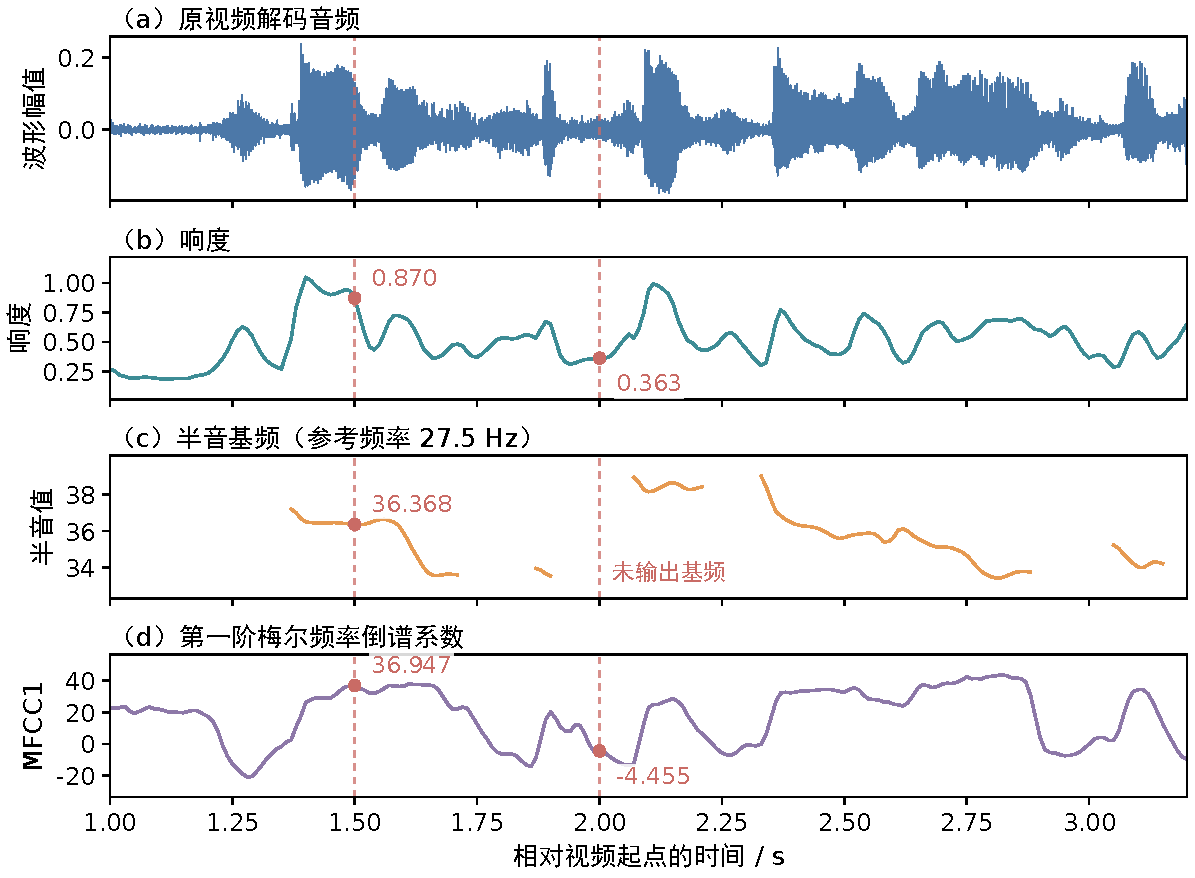
\includegraphics[width=\textwidth]{figures/fig_5_3_acoustic_example.pdf}
    \caption{同一语音片段的波形与声学特征}
    \label{fig:p1_acoustic_example}
\end{figure}

表~\ref{tab:p1_acoustic_example}列出了图中两组观测的具体数值。两条记录均具有有效音频观测，但第二条没有基频输出，说明声学记录的有效性与某一描述量是否得到估计应分别判断。该区间的响度和MFCC仍提供可用声学信息；MFCC的负值属于正常的投影结果，不能解释为能量为负。

\begin{table}[H]
    \centering\small
    \caption{两组声学观测的数值与有效性对照}
    \label{tab:p1_acoustic_example}
    \setlength{\tabcolsep}{6pt}
    \renewcommand{\arraystretch}{1.12}
    \ifdefined\pOneCompactTableBox\else\newsavebox{\pOneCompactTableBox}\fi
    \begin{lrbox}{\pOneCompactTableBox}
    \begin{tabular}{cccccc}
        \toprule
        记录区间/s & 中心时刻/s & 响度 & 半音基频 & MFCC1 & 记录有效\\
        \midrule
        $[1.49,1.51]$ & 1.50 & 0.870 & 36.368 & 36.947 & 是\\
        $[1.99,2.01]$ & 2.00 & 0.363 & $0^{\ast}$ & $-4.455$ & 是\\
        \bottomrule
    \end{tabular}
    \end{lrbox}
    \usebox{\pOneCompactTableBox}
\par\smallskip
\parbox{\wd\pOneCompactTableBox}{\footnotesize 注：$0^{\ast}$表示未输出有声基频时保留的零标记，不作为实际音高解释。}
\end{table}

为使局部声学观测进一步参与词级对齐，按输出顺序保存各时刻的25维向量。设第$m$个声学向量为$\boldsymbol a_m\in\mathbb R^{25}$，共有$N_a$条记录，则原生声学特征矩阵为
\begin{equation}
    A=\begin{bmatrix}
        \boldsymbol{a}_1^{\mathsf T}\\[4pt]
        \boldsymbol{a}_2^{\mathsf T}\\[4pt]
        \vdots\\[2pt]
        \boldsymbol{a}_{N_a}^{\mathsf T}
    \end{bmatrix}
    \in\mathbb{R}^{N_a\times25}.
    \label{eq:p1_audio_features}
\end{equation}
每行特征另关联工具返回的起止时间与观测有效标记，时间和标记均不计入25维特征。输出时间区间用于组织特征记录，而不同描述量内部采用的分析窗长并不相同，部分描述量还经过时间平滑。因此，后续将返回区间作为声学记录的时间支持近似，而不将其解释为所有描述量共同依赖的完整波形范围。

此时，矩阵$A$的每行对应一条声学记录，尚未与文本中的词一一对应。在后续词级时序对齐阶段，本文将根据候选词区间与声学记录区间的时间交叠关系进行加权聚合，形成与词级文本特征对应的声学表示。




% \subsubsection{基于eGeMAPSv02的声学低层描述量}

% 语音情感可通过响度、音高、声质及频谱形态等变化体现。为保留这些量的时间变化，本文使用openSMILE的eGeMAPSv02低层描述量（Low-Level Descriptors，LLD），在工具原生分析窗口上提取25维声学特征，而非采用整段汇总的88维统计特征\cite{stepone-ref4}。各类特征及其表征作用见表~\ref{stepone:tab1}。

% \begin{table}[H]
% \centering\small
% \caption{声学特征的组成与含义}\label{stepone:tab1}
% \begin{tabularx}{\linewidth}{@{}p{1.9cm}p{.6cm}X p{4cm}@{}}
% \toprule
% 特征组 & 维数 & 本次输出的具体内容 & 表征作用 \\
% \midrule
% 响度 & 1 & Loudness & 声音强弱变化 \\
% 频谱形态 & 5 & alphaRatio、Hammarberg指数、两个频带斜率、spectralFlux & 频谱能量分布与变化 \\
% 倒谱 & 4 & MFCC第1至第4维 & 低阶谱包络特征 \\
% 音高 & 1 & 相对27.5 Hz的F0半音值 & 韵律与音高起伏 \\
% 声质 & 3 & jitter、shimmer、HNR & 周期、振幅扰动与谐噪特性 \\
% 谐波相对幅度 & 2 & H1–H2、H1–A3 & 发声谱结构 \\
% 共振峰 & 9 & F1至F3的频率、带宽及相对F0幅度 & 声道共振形态 \\
% 合计 & 25 & 保留工具返回的完整特征名称及顺序 & 形成逐窗口声学向量 \\
% \bottomrule
% \end{tabularx}
% \end{table}

% 声学分析窗口的起止时间直接采用openSMILE输出，并加上音频起始偏移量。本文另计算窗口内均方根幅值RMS，当其低于0.0031623，即约-50 dBFS时，标记为低能量窗口。低能量只描述幅值状态，不等于缺少音频或严格的非语音判断；音频覆盖不完整、窗口为空或特征出现非有限值时，才相应设置无效观测标记。

\subsubsection{基于MediaPipe的视觉特征提取}

视觉特征侧重提取面部变化线索。眉部运动、眼睑开合和嘴部形态等变化能够补充文本语义与发声方式，因此本文采用MediaPipe Face Landmarker输出的面部blendshape系数作为视觉表示。该表示具有固定的维度与字段名称，便于逐帧记录并按时间聚合，其描述范围主要是面部形态与表情变化，不覆盖画面中的全部场景信息或肢体动作。按输出字段分组，52维系数的组成及代表性含义见表~\ref{tab:p1_visual_groups}。

\begin{table}[H]
    \centering\small
    \caption{52维面部系数的分组及代表性含义}
    \label{tab:p1_visual_groups}
    \setlength{\tabcolsep}{6pt}
    \renewcommand{\arraystretch}{1.12}
    \ifdefined\pOneCompactTableBox\else\newsavebox{\pOneCompactTableBox}\fi
    \begin{lrbox}{\pOneCompactTableBox}
    \begin{tabular}{l>{\raggedright\arraybackslash}p{16em}>{\raggedright\arraybackslash}p{11em}c}
        \toprule
        分组 & 代表性输出 & 主要描述内容 & 维度\\
        \midrule
        额眉部 & 压眉、内侧抬眉、外侧抬眉 & 眉部位置与形态 & 5\\
        眼部 & 眨眼、睁大、眯眼及视线方向 & 眼睑状态与眼部运动 & 14\\
        面颊与鼻部 & 鼓腮、面颊收紧、鼻部牵动 & 面中部形态 & 5\\
        嘴部 & 嘴角上扬或下压、噘嘴、嘴唇收紧等 & 嘴唇及嘴角形态 & 23\\
        下颌 & 张嘴、下颌前伸及左右移动 & 下颌位置与开合 & 4\\
        其他输出项 & 工具字段\_neutral & 保留输出，不作为中性情感判据 & 1\\
        \midrule
        合计 & & & 52\\
        \bottomrule
    \end{tabular}
    \end{lrbox}
    \usebox{\pOneCompactTableBox}
\end{table}

本文采用预训练模型提取面部表情特征，处理过程包括人脸检测、面部关键点估计和表情系数预测。对于第$m$个抽样画面，先检测人脸并估计面部关键点，再根据选定人脸的关键点信息预测52维表情系数，记为$\boldsymbol{c}_m\in\mathbb{R}^{52}$。

向量$\boldsymbol{c}_m$的各分量描述相应面部形态的激活程度，多个分量可以同时取较高值，因此该向量不表示互斥情感类别的概率分布。

本文保留各系数的连续输出，而不将其转换为单一表情类别，以记录多个面部部位的共同变化及其随时间的变化幅度。对于具有左右侧区分的分量，分别保留对应输出，以记录可能存在的面部运动不对称性。所有帧均采用相同的字段顺序，使同一列始终对应同一种面部描述量，为后续按词区间聚合提供一致的特征含义。

对预处理得到的抽样帧逐帧进行检测，不在帧间额外引入跟踪或平滑。当同一画面检测到多张人脸时，根据关键点包围区域的面积选择最大人脸作为当前帧的特征来源。这是一项统一的选择规则，并不保证所选人脸一定属于说话者。对于没有获得可用面部特征的画面，保留该帧位置，以零向量占位并设置无效标记，避免将观测缺失解释为中性表情。设视觉观测有效标记为$o_m^{(V)}\in\{0,1\}$，保存的视觉特征为
\begin{equation}
    \boldsymbol{v}_m=
    \begin{cases}
        \boldsymbol{c}_m, & o_m^{(V)}=1,\\
        \boldsymbol{0}, & o_m^{(V)}=0.
    \end{cases}
    \label{eq:p1_visual_observation}
\end{equation}
有效帧中某个系数较低，表示该分量的模型输出较低；无效帧中的全零向量仅用于占位，不能作为实际面部观测参与聚合。

为区分面部系数变化与观测缺失，选取样本-wny0OAz3g8\$\_\$9，将实际抽样画面与张嘴、左右嘴角上扬及左右眼睑闭合系数置于同一时间轴上，如图~\ref{fig:p1_visual_example}所示。该样本共包含31个抽样帧，其中29帧获得可用面部特征。

图中曲线直接读取已有输出，各数据点对应抽样帧，连线仅辅助观察变化，缺失位置以断线表示。竖向虚线标示上方四帧的实际时刻，底部标记显示各抽样时刻的观测有效性。该例仅用于说明特征含义与缺失处理，不代表全体样本的检测表现。

\begin{figure}[htbp]
    \centering
    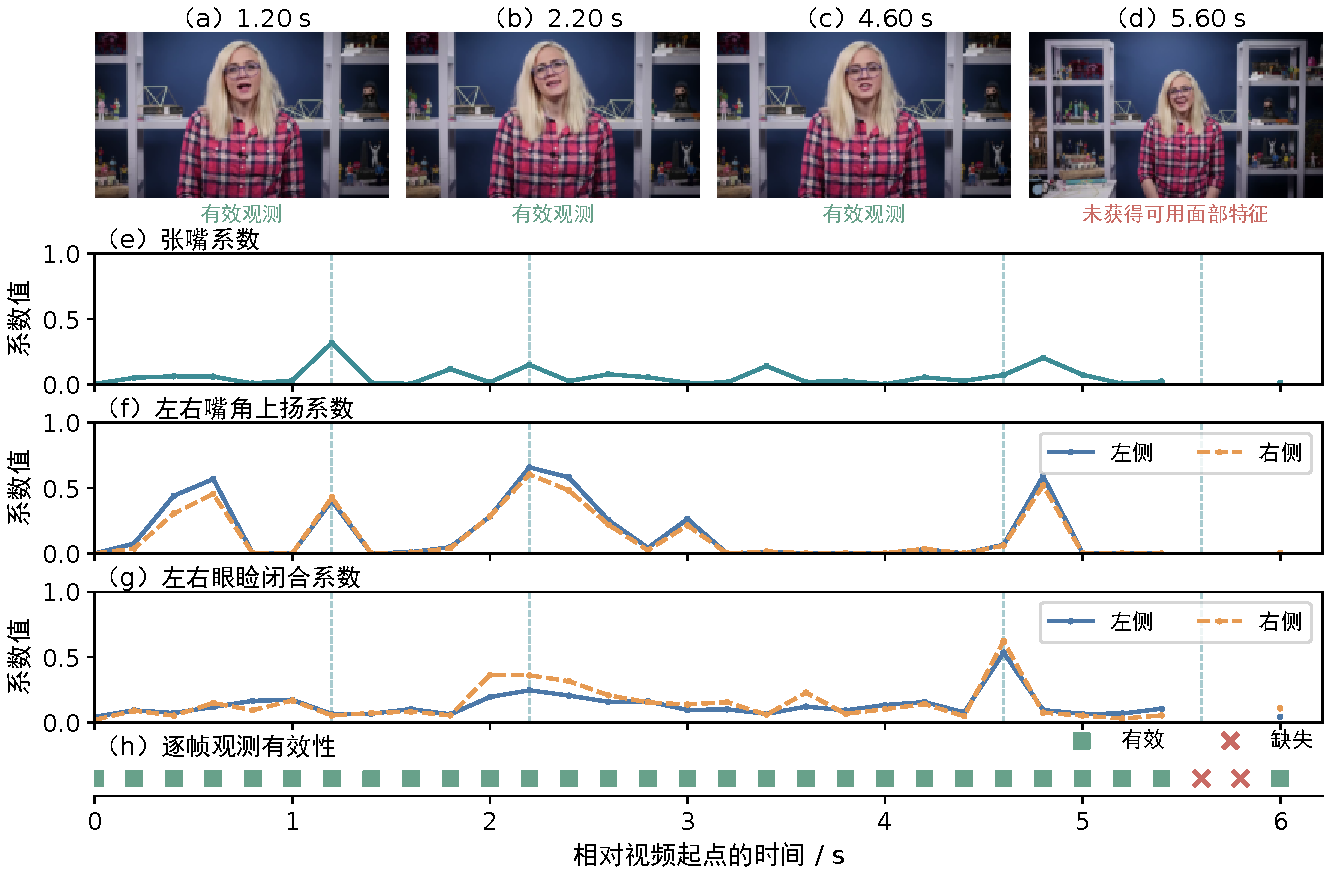
\includegraphics[width=\textwidth]{figures/fig_5_3_visual_example.pdf}
    \caption{面部系数变化与观测有效性示例}
    \label{fig:p1_visual_example}
\end{figure}

在1.20 s处，张嘴系数为0.318，对应画面中可见的张口形态；在2.20 s处，左右嘴角上扬系数分别为0.659和0.605；在4.60 s处，左右眼睑闭合系数分别升至0.535和0.623。不同系数在不同位置呈现变化，说明保留多维连续表示能够分别记录各面部部位的运动线索。这些数值描述模型对面部形态的输出，不能直接解释为某种情感的概率。

在5.60 s和5.80 s处，工具未获得可用面部特征，因而对应位置的观测标记为0。图中5.60 s的画面仍可见人物，表明“未获得可用面部特征”不能直接等同于“画面无人”。这两帧的占位零向量不作为表情变化绘入曲线，也不参与后续有效特征的加权聚合。

按抽样顺序排列后，得到原生视觉特征矩阵$V\in\mathbb{R}^{N_v\times52}$，其中$N_v$为抽样帧数。每行特征另关联实际时间戳$t_m^{(V)}$、原视频帧索引和观测有效标记，使各行能够回溯至具体画面。时间及有效标记均不计入52维特征，后续聚合时与特征矩阵共同使用。

综合三条特征提取支路，每条视频形成词级文本表示、窗口级声学表示和帧级视觉表示：
\begin{equation}
    X^{(T)}\in\mathbb{R}^{L\times768},\qquad
    A\in\mathbb{R}^{N_a\times25},\qquad
    V\in\mathbb{R}^{N_v\times52}.
    \label{eq:p1_native_features}
\end{equation}
其中$L$、$N_a$和$N_v$分别为词数、声学记录数和抽样视频帧数。三个矩阵的行具有不同的组织单位，尚不能直接按序列位置对应。下一节将结合给定转写与音频估计词级时间边界，再依据时间交叠关系聚合有效声学与视觉特征，建立统一词位置的三模态表示。


% \subsubsection{基于MediaPipe的面部表情系数}

% 视觉部分采用MediaPipe Face Landmarker，对抽样帧输出52维blendshape系数\cite{stepone-ref5}，包括眉部、眼部、下颌、嘴部及鼻部等表情形变参数。本文保留模型原生系数，例如mouthSmileLeft、mouthSmileRight、jawOpen和browInnerUp，以描述局部面部运动。该输出与OpenFace的FACS动作单元含义不同，也不是情感类别的预测概率。

% 检测采用IMAGE模式，最小人脸检测置信度与人脸存在置信度均设为0.5，最多检测两张人脸。若一帧出现多脸，则选择面部关键点包围区域面积最大者，并记录人脸数量；此规则未进行说话者身份验证。未检出可用面部特征时，保存零向量和False掩码。零向量在此仅用于占位，不能解释为中性表情。

% 为使离散视觉观测参与区间运算，以相邻抽样PTS的中点作为时间单元边界。首尾分别延伸到片段起止时刻，每个单元采用对应抽样帧的表情系数。该近邻保持规则明确了5 Hz离散采样的时间支持范围，但不意味着单元内部表情真实不变，也不能覆盖更快的微表情变化。


\subsection{三模态特征的词级时序对齐}


上一节分别获得了词级文本特征、窗口级声学特征和帧级视觉特征。然而，三类特征的行索引具有不同含义：文本特征按原文词序排列，声学特征对应短时音频记录，视觉特征对应抽样视频帧。因此，即使属于同一条视频，三个特征矩阵中相同行号的记录也未必对应同一时间段，尚不能直接按行建立三模态对应关系。

为此，本文以原始转写中的词为共同组织单位，分两步完成时序对齐。首先，利用给定转写与音频进行基于CTC的强制对齐，估计每个词在音频中的起止时间。该步骤建立文本词与音频时间之间的联系，为后续特征聚合提供词级时间区间。其次，由于声学记录与视频帧均保留了相对于视频起点的时间信息，可将它们与词级时间区间置于同一时间轴上，并依据时间交叠关系及观测有效性，对声学和视觉特征分别进行加权聚合。

经过上述处理，每个词均关联其文本表示及对应时间区间内的声学、视觉表示，三类特征由不同粒度的序列转化为具有相同词序的特征矩阵。对于缺少有效声学或视觉观测的词位置，保留相应的无效标记；词级时间边界的可靠性则在后续样本质量核验中进一步评估。


\subsubsection{基于CTC的文本与音频词级强制对齐}

给定转写提供了词的内容及排列顺序，但没有说明每个词在音频中的出现时间。因此，本节的任务是在已知文本的条件下，确定各词对应的起止时间。本文首先利用预训练的 Wav2Vec2 模型估计音频各输出时刻的字符概率，再通过连接时序分类（Connectionist Temporal Classification，CTC）约束下的强制对齐，建立文本字符与音频时间之间的对应关系，最后将字符时间位置合并为词级时间区间。

本文采用第~\ref{sjycl}~节构建的规范化转写文本作为对齐目标，并保留其中字符与原文词之间的映射关系。由此，后续获得的字符时间位置能够合并回对应的原文词，使词级时间区间与已有文本特征保持一致的词索引。

将预处理后的单声道音频输入 Wav2Vec2，得到各输出时刻对应的字符概率。记 $p_r(c)$ 为第 $r$ 个输出时刻对应字符 $c$ 的概率，其中候选符号除文字字符和词界符外，还包括CTC空白符 $\varnothing$。空白符表示该时刻不输出目标字符，不直接等同于音频中的静音。模型在此过程中保持参数固定，仅用于提供字符概率。

由于一个字符可能持续多个输出时刻，文本字符与模型输出之间并非一一对应。CTC允许同一字符连续重复出现，也允许路径中包含空白符。如图~\ref{fig:p1_ctc_principle}所示，给定词\texttt{HELLO}对应的示例路径可以多次输出\texttt{H}或\texttt{L}。先合并连续重复符号，再删除空白符，即可还原字符序列。其中，两组\texttt{L}由空白符分隔，因此在折叠后仍保留为两个字母，最终得到\texttt{HELLO}。

保留字符在原始路径中的时间位置，可确定图示词的候选时间区间$[t_1,t_{13}]$。图中字符位置与时间刻度均为示例，仅用于说明路径折叠与时间定位过程。

\begin{figure}[htbp]
    \centering
    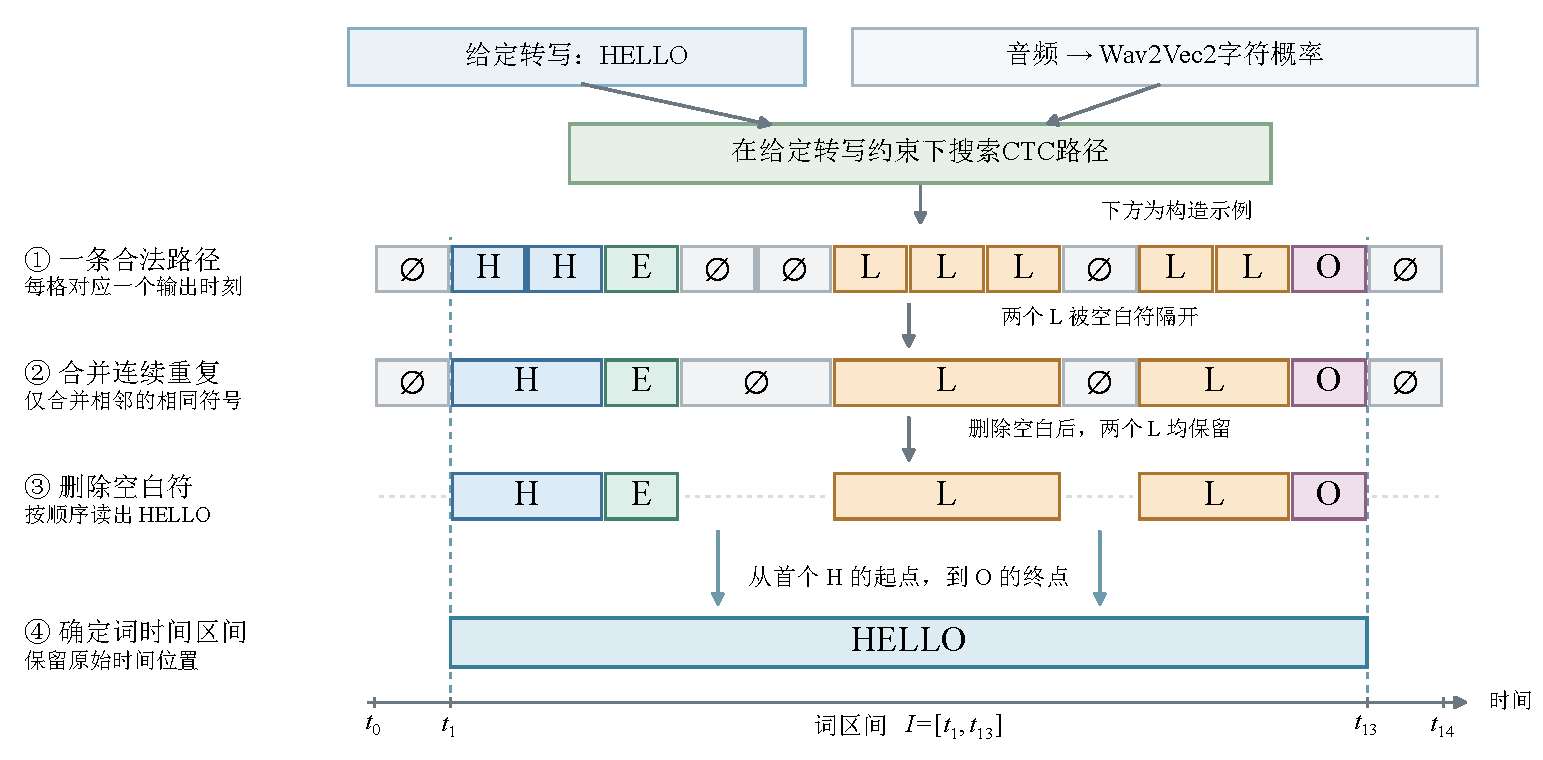
\includegraphics[width=\textwidth]{figures/fig_5_4_ctc_principle.pdf}
    \caption{CTC路径折叠与词级时间定位示意}
    \label{fig:p1_ctc_principle}
\end{figure}

上述合并与删除操作用于判断一条路径是否与给定文本一致，并不丢弃字符原先对应的时间位置。对于同一段转写，通常存在多条满足条件的路径。本文根据音频的字符概率，从中选择整体概率最大的一条。设规范化后的目标字符序列为 $\boldsymbol{y}$，模型共有 $R$ 个输出时刻，路径为
$\boldsymbol{\pi}=(\pi_1,\ldots,\pi_R)$，并用
$\mathcal{B}$ 表示先合并连续重复符号、再删除空白符的操作，则最优路径为
\begin{equation}
\boldsymbol{\pi}^{*}
=
\underset{
\boldsymbol{\pi}:\,
\mathcal{B}(\boldsymbol{\pi})=\boldsymbol{y}
}{\arg\max}
\sum_{r=1}^{R}\log p_r(\pi_r).
\label{eq:p1_ctc_optimal_path}
\end{equation}
其中，约束
$\mathcal{B}(\boldsymbol{\pi})=\boldsymbol{y}$
保证路径还原后的字符内容与顺序符合给定转写，目标函数则用于比较这些合法路径对音频的匹配程度。本文采用动态规划求解，并通过回溯获得各目标字符对应的输出时刻。

得到字符位置后，依据模型输出的时间步长及音频起点偏移，将这些位置统一转换到以视频起点为原点的时间轴上。随后，根据字符与原文词之间的映射，取每个词首个文字字符的起点与末个文字字符的终点，形成该词的候选时间区间。

具体地，设 $\mathcal{R}_k$ 为最优路径中分配给第 $k$ 个原文词所属文字字符的输出时刻索引集合，不包含空白符与词界符；第 $r$ 个输出时刻对应的时间区间为 $[a_r,b_r]$。当 $\mathcal{R}_k$ 非空时，定义
\begin{equation}
I_k=[s_k,e_k],
\qquad
s_k=\min_{r\in\mathcal{R}_k}a_r,
\qquad
e_k=\max_{r\in\mathcal{R}_k}b_r.
\label{eq:p1_ctc_word_interval}
\end{equation}
例如，图~\ref{fig:p1_ctc_principle}中，
HELLO 的时间区间从首个 H 的起点延伸至
O 的终点。词内部的空白位置包含在该区间内，首尾之外的空白位置则不纳入。因此，相邻词的区间不必首尾相接。

在保存词时间区间的同时，本文记录相应的对齐置信度，供后续质量核验使用。若无法获得覆盖给定转写的合法路径，或某个词没有对应的字符时刻，则标记对齐失败，不以均匀分配时间的方式补造词边界。

经过上述处理，原文中的词获得了候选时间区间，并保持与词级文本特征相同的词索引。下一步将以这些区间为共同参照，根据时间交叠关系聚合声学与视觉特征，使三种模态在同一词位置上建立对应关系。



\subsubsection{基于词时间区间的声学与视觉特征加权聚合}

上一节获得了各词的候选时间区间，但声学特征仍按短时记录排列，视觉特征仍对应离散视频帧。为使它们与词级文本特征逐行对应，本文以词时间区间为共同参照，将与该区间存在时间交叠的有效声学和视觉观测分别进行加权聚合。交叠时间越长，表示该条观测在时间上与当前词的关联范围越大，因此赋予其更高的聚合权重。

首先，需要明确每条声学与视觉记录所代表的时间区间。对于声学特征，采用提取工具返回的起止时间，并统一到以视频起点为原点的时间轴上。由于不同声学描述量内部采用的分析窗长及平滑方式不完全相同，该区间作为声学记录的时间支持近似，不将其解释为全部描述量共同依赖的完整波形范围。

对于视觉特征，抽样帧本身仅具有时间戳，需要进一步构造其代表的时间区间。本文以相邻抽样帧时间戳的中点作为分界，使每帧代表时间上距离它最近的一段画面。设抽样帧时间戳依次为
$t_1^{(V)},\ldots,t_{N_v}^{(V)}$，片段总时长为 $T$，定义区间边界
\begin{equation}
b_0=0,\qquad
b_j=\frac{t_j^{(V)}+t_{j+1}^{(V)}}{2},
\quad j=1,\ldots,N_v-1,\qquad
b_{N_v}=T,
\label{eq:p1_visual_support_edges}
\end{equation}
则第 $j$ 帧的代表区间为
$J_j^{(V)}=[b_{j-1},b_j]$。
这一处理将离散帧转换为可计算时间交叠的区间，是对帧间视觉状态的近似表示，并不意味着表情在整个区间内完全不变。

为直观说明加权过程，图~\ref{fig:p1_overlap_principle}
以三条视觉记录为例。假设某词的候选时间区间为
$[1.00,1.45]$（图中虚线范围），与三帧代表区间的交叠时长
分别为 $0.10\,\mathrm{s}$、$0.20\,\mathrm{s}$ 和
$0.15\,\mathrm{s}$。其中第二帧（图中灰色斜线区域）没有可用面部特征，
因此不参与聚合。将其余两条有效观测记录（图中草绿色区域）的交叠时长归一化，
得到权重 $0.4$ 和 $0.6$，该词的视觉特征即为
$\widehat{\boldsymbol{v}}
=0.4\boldsymbol{v}_1+0.6\boldsymbol{v}_3$。
声学特征采用相同规则单独聚合，已有的词级文本特征保持不变。

\begin{figure}[htbp]
    \centering
    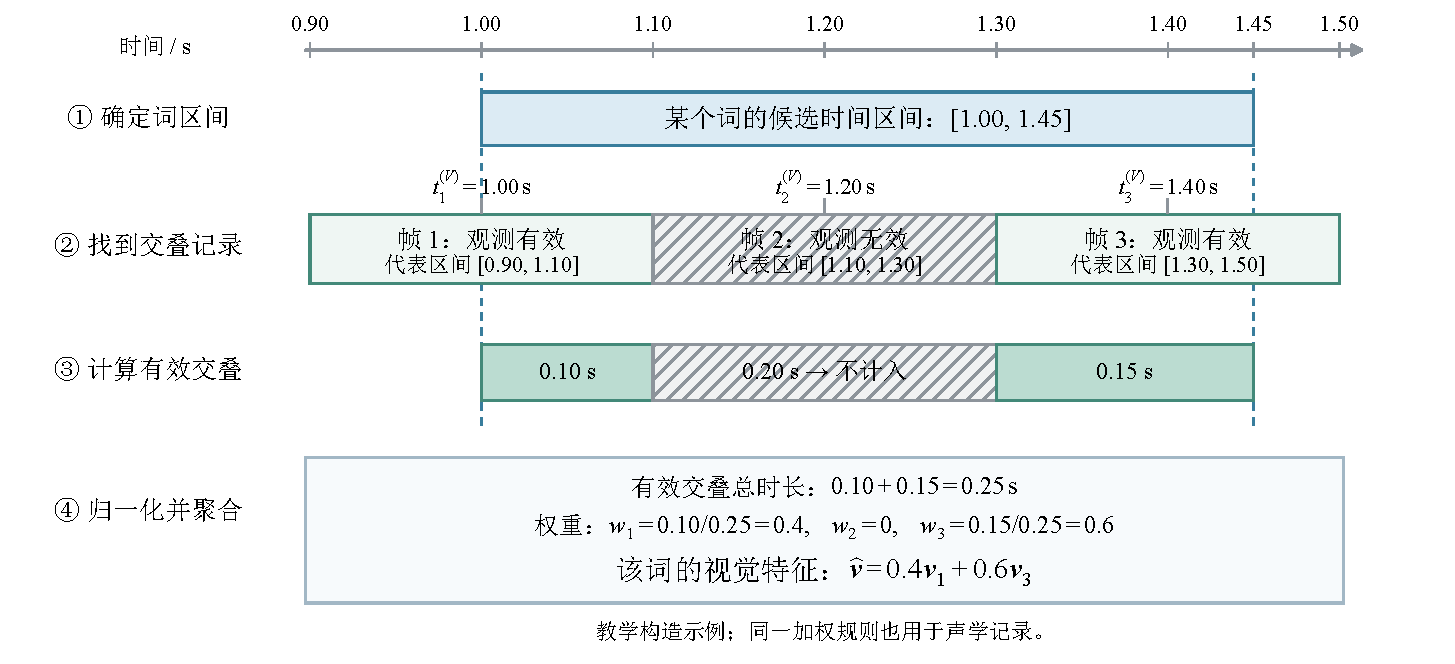
\includegraphics[width=\textwidth]
    {figures/fig_5_4_overlap_principle.pdf}
    \caption{基于词时间区间的加权聚合示意图}
    \label{fig:p1_overlap_principle}
\end{figure}

为统一描述两种模态，记
$M\in\{A,V\}$ 分别表示声学与视觉模态，
$\boldsymbol{x}_j^{(M)}$ 为第 $j$ 条原生特征，
$J_j^{(M)}=[u_j^{(M)},v_j^{(M)}]$ 为其对应时间区间，
$o_j^{(M)}\in\{0,1\}$ 为观测有效标记。
对于第 $k$ 个词的时间区间 $I_k=[s_k,e_k]$，
其与第 $j$ 条记录的有效交叠时长定义为
\begin{equation}
d_{kj}^{(M)}
=
o_j^{(M)}
\max\left\{
0,\,
\min\bigl(e_k,v_j^{(M)}\bigr)
-
\max\bigl(s_k,u_j^{(M)}\bigr)
\right\}.
\label{eq:p1_overlap_duration}
\end{equation}
当两个区间不相交，或该条观测无效时，
$d_{kj}^{(M)}=0$，相应特征不参与聚合。
例如，没有获得可用人脸特征的视频帧即使落在词区间内，也不会将其占位零向量计入有效观测的平均值。

将同一词对应的有效交叠时长归一化，得到聚合权重：
\begin{equation}
D_k^{(M)}=\sum_{j=1}^{N_M}d_{kj}^{(M)},
\qquad
w_{kj}^{(M)}
=
\begin{cases}
\dfrac{d_{kj}^{(M)}}{D_k^{(M)}},
& D_k^{(M)}>0,\\[6pt]
0,
& D_k^{(M)}=0,
\end{cases}
\label{eq:p1_overlap_weight}
\end{equation}
其中，$N_A=N_a$、$N_V=N_v$，分别为声学记录数与抽样帧数。
当存在有效交叠时，同一词在同一模态下的聚合权重之和为1。
例如，若某词仅与两条有效视觉记录发生交叠，
交叠时长分别为$0.06\,\mathrm{s}$和$0.14\,\mathrm{s}$，
则归一化后的权重分别为$0.3$和$0.7$。

据此，第 $k$ 个词对应的聚合特征及观测有效标记为
\begin{equation}
\widehat{\boldsymbol{x}}_k^{(M)}
=
\sum_{j=1}^{N_M}
w_{kj}^{(M)}\boldsymbol{x}_j^{(M)},
\qquad
\widehat{o}_k^{(M)}
=
\begin{cases}
1, & D_k^{(M)}>0,\\
0, & D_k^{(M)}=0.
\end{cases}
\label{eq:p1_word_pooled_feature}
\end{equation}
若某词区间内没有有效观测，则聚合结果为零向量，并设置无效标记。
因此，后续使用特征时需要同时读取该标记，不能仅凭零值判断声音或面部表情的状态。
对于未获得有效候选时间区间的词，也保留其原有词位置，并将相应聚合结果标记为无效。

需要说明的是，声学记录的时间区间可能相互重叠，因此
$D_k^{(A)}$ 是各条记录与词区间的交叠时长之和，可能大于词本身的持续时间。
它仅用于归一化聚合权重，不等同于有效音频覆盖时长。
此外，一条原生记录若与相邻两个词均有交叠，可以分别参与两个词的聚合，无须被强行划归其中一个词。

按原文词序排列聚合结果后，每条样本得到
\begin{equation}
X^{(T)}\in\mathbb{R}^{L\times768},
\qquad
\widehat{A}\in\mathbb{R}^{L\times25},
\qquad
\widehat{V}\in\mathbb{R}^{L\times52},
\label{eq:p1_aligned_feature_matrices}
\end{equation}
其中，$L$ 为原文词数，词级文本特征 $X^{(T)}$ 保持不变。
三个矩阵的第 $k$ 行均对应第 $k$ 个原文词，从而建立统一词位置的三模态表示。
同时保留词时间区间、参与聚合的原生记录索引、聚合权重及观测有效标记，使词级特征能够回溯至对应的音频记录和视频帧。

上述聚合建立了三种模态在词位置上的对应关系，但观测有效并不意味着词时间边界一定可靠。
例如，某词区间内可能存在可用人脸，而该词的时间定位置信度仍然较低。
因此，后续样本质量核验将分别检查观测有效性与对齐时间质量，为聚合结果的使用提供依据。

% 实验结果分析：完整替换稿，表格代码均已内嵌。
% 导言区依赖：amsmath、amssymb、graphicx、float、array、booktabs、longtable、url。
% 图片路径沿用 figures/；不要与“问题一_全部表格.tex”重复载入。
\subsection{实验结果分析}
\label{sec:p1_results}
\urlstyle{same}

前文已通过三模态特征提取、CTC强制对齐与时间交叠加权，将原始视频及给定转写转化为具有统一词位置的特征序列。本节进一步检验这些输出能否回应赛题提出的原始样本覆盖完整性、时序组织可核验性，以及方法合理性与可复现性要求。具体而言，先核对样本及模态观测的覆盖范围，再依次通过自动诊断、固定窗口对照与人工审核，考察候选对应的筛选范围、时间划分的影响及输入异常的来源；随后以典型样本验证特征与原始素材之间的映射，最后给出全部100条样本的结果汇总、文件读取方式和复现流程。由此，将前文的方法定义落实为能够逐样本查阅、按记录复算的特征输出。

\subsubsection{样本覆盖完整性与特征有效性}
\label{sec:p1_quality_scope}

为检查原始样本覆盖完整性，本文以视频编号和片段编号组成的唯一标识，核对原始视频、给定转写、标签记录与输出目录。已有全量核验结果表明，附件1的100条样本均具有对应输出，原文及标签与输入记录一致，源视频哈希核对通过。各样本分别生成768维文本、25维声学和52维视觉词级特征，三种矩阵的行数均等于该样本的原文词数，共保留1932个词位置，未发生长度截断。表~\ref{tab:p1_result_overview}在样本覆盖的基础上进一步统计各模态的观测状态，其中样本比例以100为分母，词比例以1932为分母。

\begin{table}[H]
    \centering\small
    \caption{样本处理与三种模态的观测覆盖情况}
    \label{tab:p1_result_overview}
    \setlength{\tabcolsep}{6pt}
    \renewcommand{\arraystretch}{1.12}
    \ifdefined\pOneCompactTableBox\else\newsavebox{\pOneCompactTableBox}\fi
    \begin{lrbox}{\pOneCompactTableBox}
    \begin{tabular}{lrr}
        \toprule
        统计项目 & 数量 & 占比\\
        \midrule
        已处理样本 & 100 & 100.00\%\\
        与原文对应的输出词位置 & 1932 & 100.00\%\\
        文本模态可观测的词 & 1932 & 100.00\%\\
        声学模态可观测的词 & 1932 & 100.00\%\\
        视觉模态可观测的词 & 1595 & 82.56\%\\
        \bottomrule
    \end{tabular}
    \end{lrbox}
    \usebox{\pOneCompactTableBox}
\par\smallskip
\end{table}

完整生成输出文件并不意味着每个词位置都具有同等充分的模态信息。前文原始画面观察已显示，部分时刻难以获得可用人脸；图~\ref{fig:p1_visual_coverage}进一步给出这一现象在全量数据中的范围。3973帧抽样画面中，3253帧获得面部特征，720帧未获得可用结果；按候选词区间聚合后，1595个词具有有效面部记录，337个词缺少相应记录。由于一帧可以参与多个词的聚合，一个词也可以关联多帧，帧级与词级覆盖率分别以各自记录总数为分母。该结果说明，视觉缺失需要作为输出状态显式保存，不能仅根据三模态矩阵是否具有相同行数判断其信息是否完整。

声学模态则呈现不同的情况：所有词位置均有可计算记录，但原生声学序列的幅度状态存在明显差异。以数字音频满幅1为基准，将短时均方根幅度（RMS）低于0.0031623的记录标记为低能量，77261条记录中共有9918条满足该条件，占12.84\%，如图~\ref{fig:p1_audio_energy_share}所示。该标记用于保留低幅度状态，不作为无语音或观测缺失的直接判据，因此不会据此删除记录或改变原文词位置。

\begin{figure}[H]
    \centering
    \begin{minipage}[b]{.48\linewidth}
        \centering
        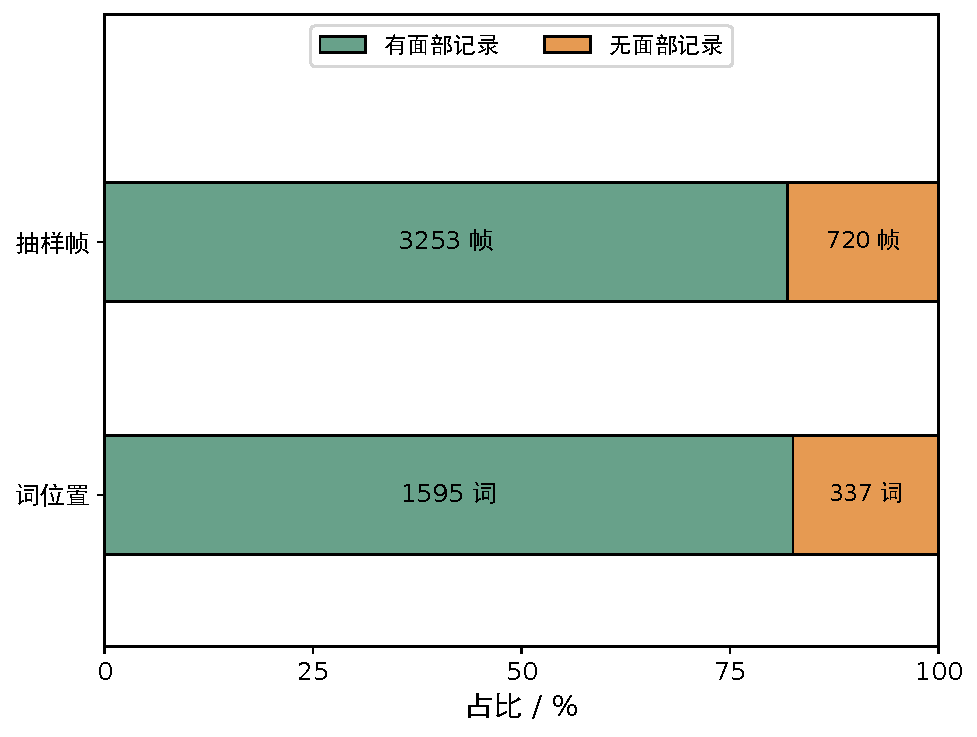
\includegraphics[width=\linewidth]{figures/fig_p1_visual_coverage_single.pdf}
        \caption{面部特征的帧级与词级覆盖}
        \label{fig:p1_visual_coverage}
    \end{minipage}\hfill
    \begin{minipage}[b]{.48\linewidth}
        \centering
        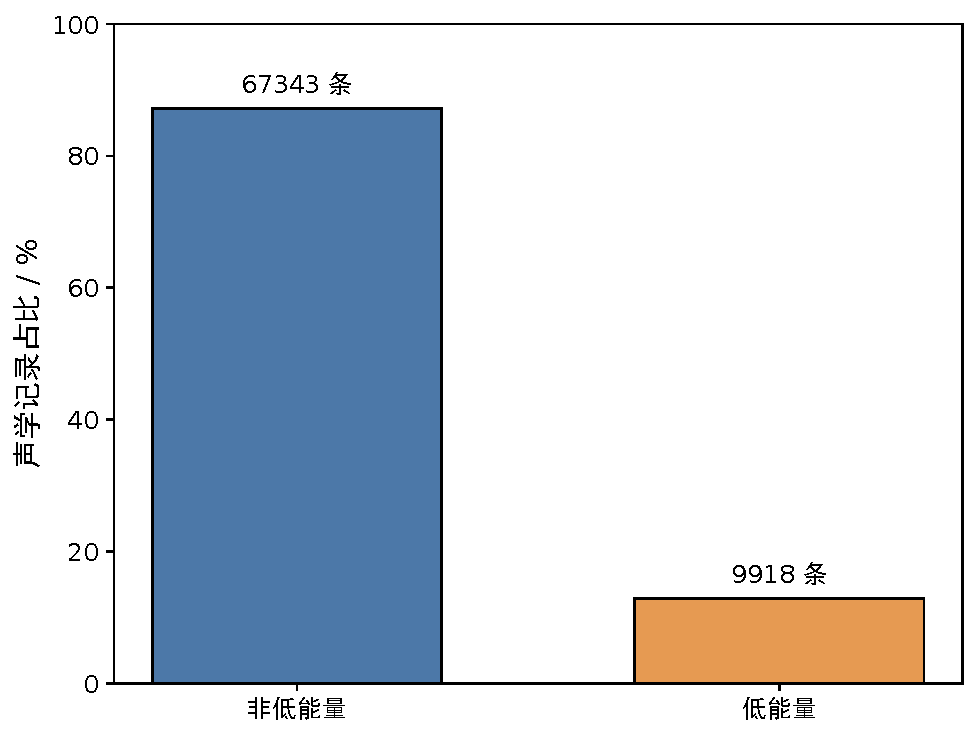
\includegraphics[width=\linewidth]{figures/fig_p1_audio_energy_share_single.pdf}
        \caption{声学记录的低能量占比}
        \label{fig:p1_audio_energy_share}
    \end{minipage}
\end{figure}

图~\ref{fig:p1_rms}与图~\ref{fig:p1_rms_zoom}以样本\nolinkurl{-iRBcNs9oI8$_$9}说明上述标记的时间分布。该样本333条RMS记录中有147条低于阈值；完整幅度图显示若干较强峰值，保持相同横轴的低幅值放大图则呈现峰值之间及片段末端的低能量区间。橙色虚线为阈值，橙点为低于阈值的记录。两图表明，声学输入状态随时间变化，采用逐记录标记能够保留整段平均统计无法呈现的局部差异。

\begin{figure}[H]
    \centering
    \begin{minipage}[b]{.48\linewidth}
        \centering
        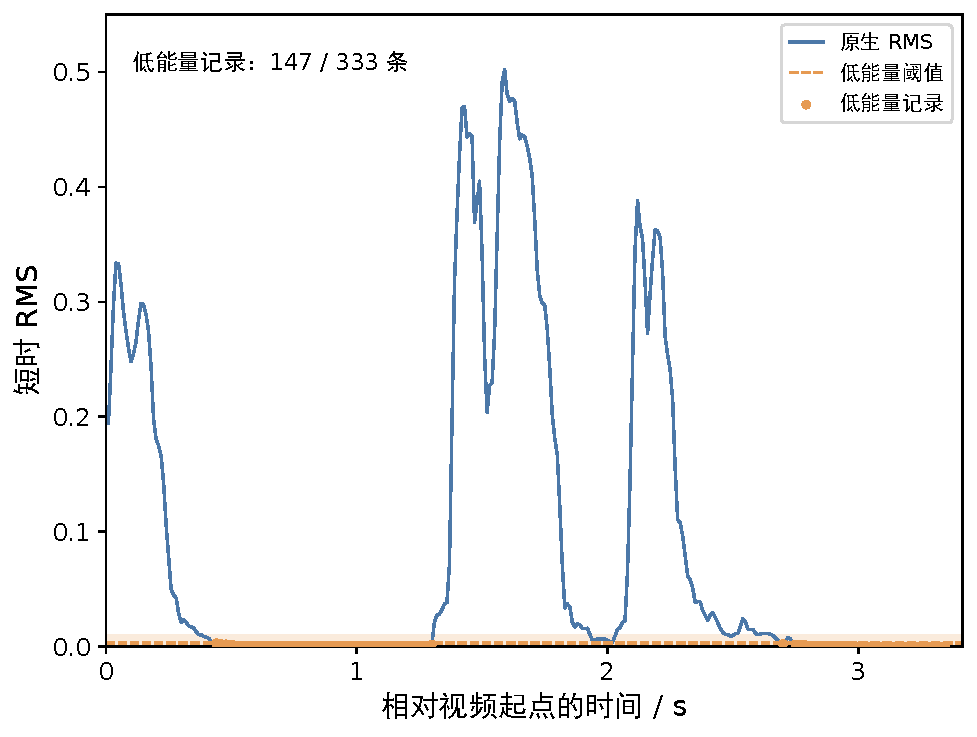
\includegraphics[width=\linewidth]{figures/fig_p1_rms_single.pdf}
        \caption{实例音频的短时RMS}
        \label{fig:p1_rms}
    \end{minipage}\hfill
    \begin{minipage}[b]{.48\linewidth}
        \centering
        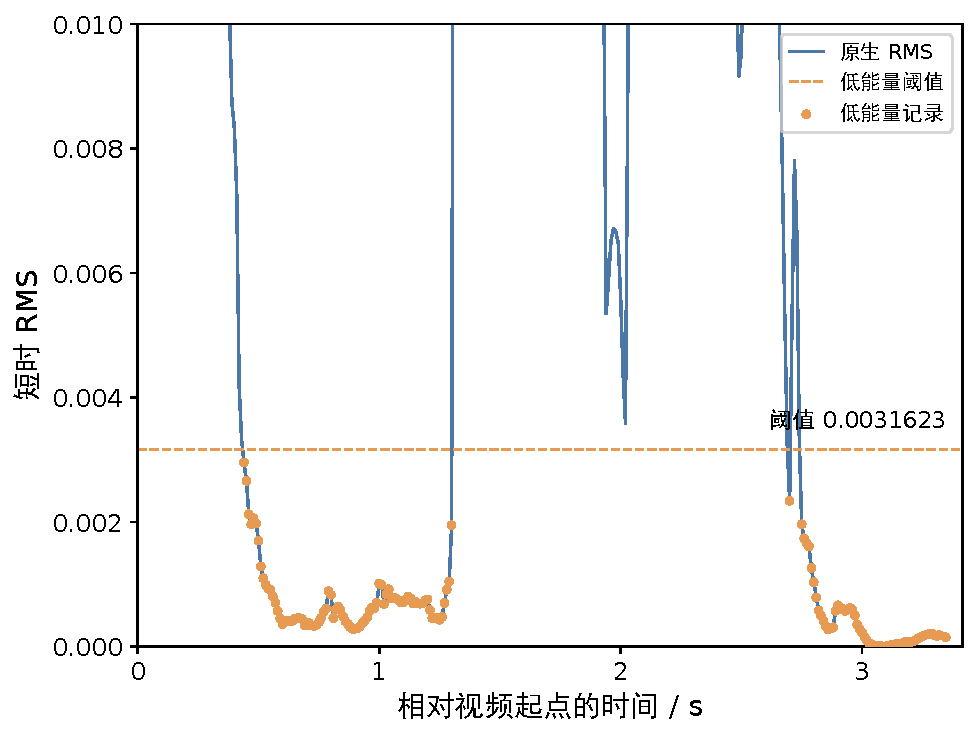
\includegraphics[width=\linewidth]{figures/fig_p1_rms_zoom_single.pdf}
        \caption{同一时间范围的低幅值放大}
        \label{fig:p1_rms_zoom}
    \end{minipage}
\end{figure}

另有两条样本的解码音频波形全为零，其声学特征各维均不随时间变化。结合视觉缺失与声学低能量结果可知，样本覆盖、模态观测和转写对应关系需要分别检查。本文保留全部样本及原始词位置，对视觉缺失采用零向量占位和无效标记，对低能量记录保留幅度状态；这种处理既维持了输入与输出的一一对应，也使异常位置能够被单独识别。在此基础上，下一步需要判断候选词时间区间是否得到实际音频的支持。

\subsubsection{时序对齐质量评估与人工审核}
\label{sec:p1_timing_quality}

前文的词级聚合以候选时间区间为依据，其可靠性直接影响哪些声学和视觉记录被分配到同一词位置。因此，时序组织的检查不能停留在矩阵行数一致，还需要评估给定转写与实际语音的匹配情况。本次CTC强制对齐为1932个词均生成候选区间，但满足字符路径约束只能说明算法获得了合法解，不能保证真实词界准确。本文据此设置局部词匹配与整段文本差异两个诊断层次，并用人工审核解释整段异常。

词级置信度取最优CTC路径中属于该词的文字字符帧概率的几何平均，不含空白符和词界符，用于描述模型对局部匹配的支持程度。片段级诊断词错误率（Word Error Rate，WER）则将无转写约束的贪心识别文本与规范化转写比较，以最少词编辑数除以参考词数，反映整段文本的差异。二者分别考察局部与整体：某些词即使得分较高，也可能处于整段内容不对应的片段中。由于两项指标来自同一声学模型，以下将其用于质量筛查，而不将其视为独立的词界准确性评价；WER包含插入操作，取值可以超过1。

图~\ref{fig:p1_ctc_confidence}与图~\ref{fig:p1_diagnostic_wer}显示，词级置信度与片段级WER均存在需要关注的异常区域。1932个词的置信度中位数为0.9585，1034个词不低于0.95，但仍有350个词低于0.1；100条片段的诊断WER均值为0.4689，其中21条超过0.8，9条超过1。图中的虚线和阴影分别标示对应阈值与关注区域。这些结果说明，整体较高的词级得分不足以支持无差别使用全部候选区间，需要进一步结合片段状态确定可用范围。

\begin{figure}[H]
    \centering
    \begin{minipage}[b]{.48\linewidth}
        \centering
        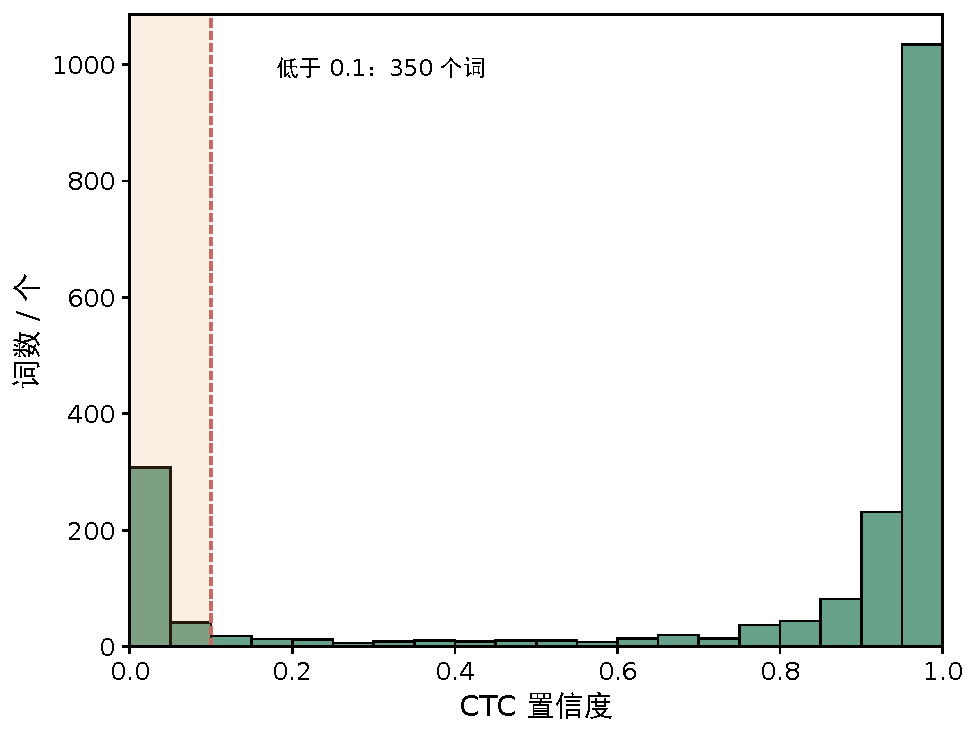
\includegraphics[width=\linewidth]{figures/fig_p1_ctc_confidence_single.pdf}
        \caption{词级CTC置信度分布}
        \label{fig:p1_ctc_confidence}
    \end{minipage}\hfill
    \begin{minipage}[b]{.48\linewidth}
        \centering
        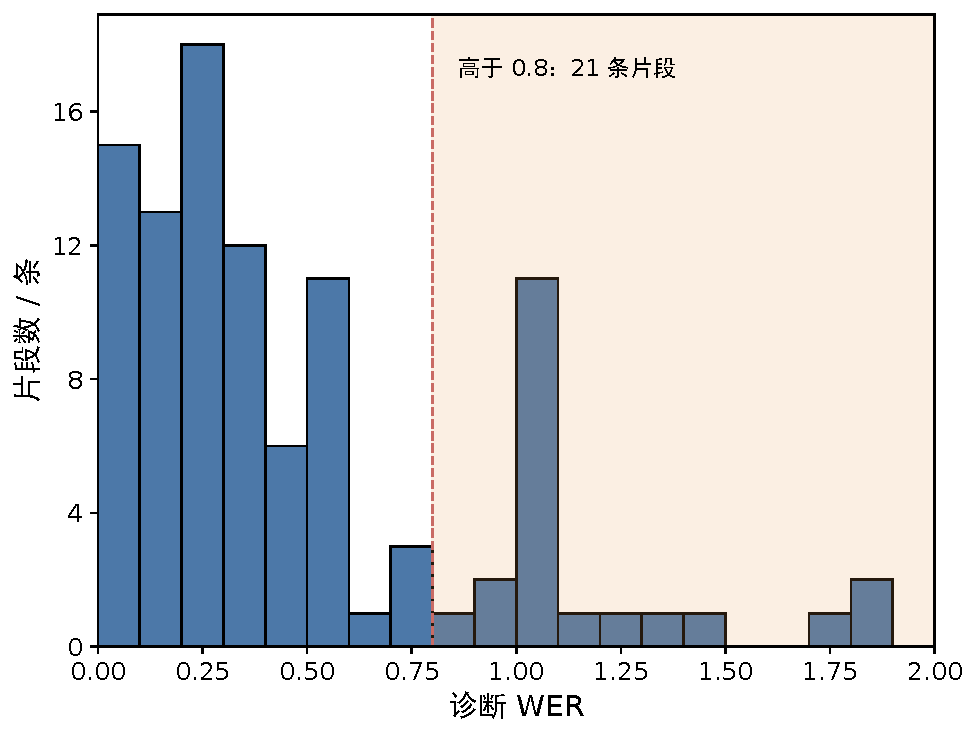
\includegraphics[width=\linewidth]{figures/fig_p1_diagnostic_wer_single.pdf}
        \caption{片段级诊断WER分布}
        \label{fig:p1_diagnostic_wer}
    \end{minipage}
\end{figure}

本文采用片段级与逐词两层筛选，将上述诊断落实为可随特征文件保存的质量标记。首先，平均词置信度低于0.2、置信度低于0.1的词超过一半、诊断WER大于0.8，或无法形成完整CTC路径的样本均列入整段复核，暂不采用其词级时间对应。其次，在其余样本中，仅将成功获得候选起止时间且置信度不低于0.1的词计为通过筛选。这些阈值作为保守检查条件，未利用情感标签或人工词界标注优化；筛选改变的是词级对应的使用标记，不删除样本、词位置或原始特征。

图~\ref{fig:p1_quality_flow}将两层筛选与模态观测检查串联起来。在100条样本中，19条的平均词置信度低于0.2，20条有超过一半的词置信度低于0.1，21条的诊断WER大于0.8，没有样本因无法形成完整CTC路径而被标记。这四项条件分别检查，每条样本只要满足其中任一项就进入整段复核；同一样本可能同时满足多项条件，因此各项数量不能直接相加。本次前两项标记的样本均已包含在WER大于0.8的21条样本中，去除重复计数后，需整段复核的仍为21条，共涉及317个词。其余79条样本包含1615个词，其中70个因置信度不足未通过逐词筛选，剩余1545个通过筛选，占全部词的79.97\%。这1545个词中，158个缺少有效面部记录，1387个同时满足对齐筛选和三模态可观测条件，占全部词的71.79\%。

\begin{figure}[H]
    \centering
    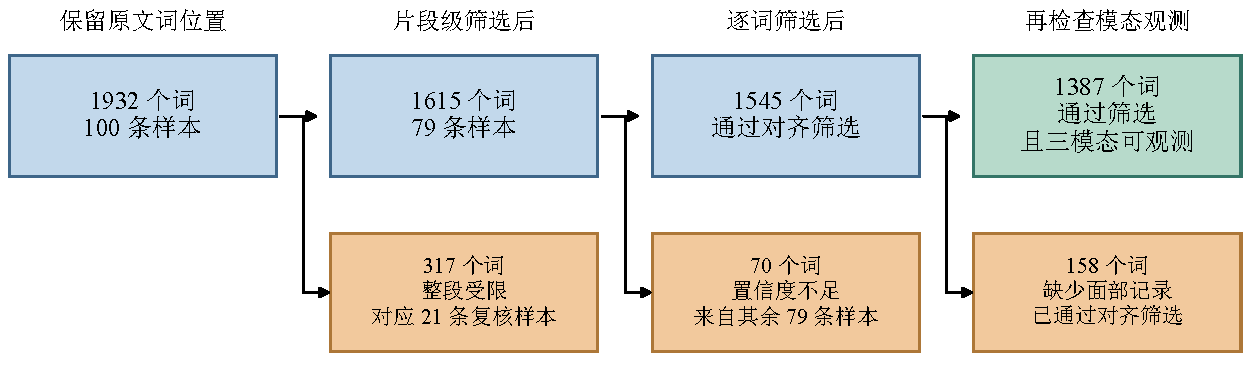
\includegraphics[width=\linewidth]{figures/fig_p1_quality_flow.pdf}
    \caption{从全部词位置到满足不同使用条件的词位置：各分支数量可逐项核对}
    \label{fig:p1_quality_flow}
\end{figure}

图中各分支均对应明确的使用条件，而非对原始数据的删减。317个整段受限词中包含37个局部置信度达到阈值的词，因而未通过筛选的387个词多于低置信度词的350个。另一方面，通过时间筛选但缺少面部记录的158个词仍保有文本与声学信息，只是不满足三模态同时可观测的条件。因此，后续读取词级输出时需要分别使用对齐质量标记与模态观测标记，区分“存在可计算记录”和“满足当前对齐筛选条件”这两种状态。

进一步将片段平均置信度阈值取0.1、0.2、0.3，诊断WER阈值取0.6、0.8、1.0，其余条件保持不变。在三种平均置信度阈值下，待复核样本数均随WER阈值变化依次为25、21、20条，表明当前数据的复核数量主要受WER条件影响。该检查反映筛选范围对阈值的敏感性，不能据此确定最优阈值或计算真实对齐准确率。

\label{sec:p1_window_analysis}
上述筛选回答了候选时间对应的使用范围，但尚未说明采用何种时间单元组织特征更便于保留信息。前文以词作为共同单位，是为了使文本语义单元与相应时段的视听记录保持明确联系。为考察统一时间切分可能带来的影响，本文在相同原生特征上构造0.2~s和0.5~s固定窗口作为补充对照，窗口均从零时刻开始，末窗截取至片段终点，并沿用有效时间交叠加权规则。该实验关注平均聚合对局部变化的保留程度，以及固定边界对词区间完整性的影响，为时间组织方式的合理性分析提供依据。

固定窗口对照包含聚合与重建两个步骤：首先分别聚合两种窗口内的原生特征，再根据时间交叠关系将窗口特征映回原生记录位置，以便与原序列比较。图~\ref{fig:p1_window_reconstruction}以响度展示重建结果，青蓝色线为原生记录，蓝线与橙线分别对应短窗和长窗。窗口平均削弱了原曲线的局部峰谷，较长窗口的平滑范围更大，说明统一时间汇总在压缩序列的同时会改变局部特征变化。这里的重建对象是特征序列，而非原始音频波形。

图~\ref{fig:p1_word_window_overlap}检查同一样本中的词区间是否被固定窗口切分。绿色线为\texttt{successful}的候选区间$[1.84247,2.40247]\,\mathrm{s}$，上、下两排分别为0.2~s和0.5~s窗口。该词分别与4个短窗和2个长窗交叠，在两种划分下均计为一个跨界词。第四个短窗的交叠仅约0.00247~s，图中以箭头注明；统计时将大于$10^{-8}\,\mathrm{s}$的交叠视为有效交叠。跨界指标只判断是否与至少两个窗口交叠，不区分交叠窗口数量及切分幅度。

上述图示采用样本\nolinkurl{-egA8-b7-3M$_$1}。其选取条件为未触发整段复核、面部观测帧占比不低于80\%，且时长最接近10~s。该样本实际时长10.266~s，包含20个词，其中18个通过对齐筛选。

\begin{figure}[H]
    \centering
    \begin{minipage}[b]{.48\linewidth}
        \centering
        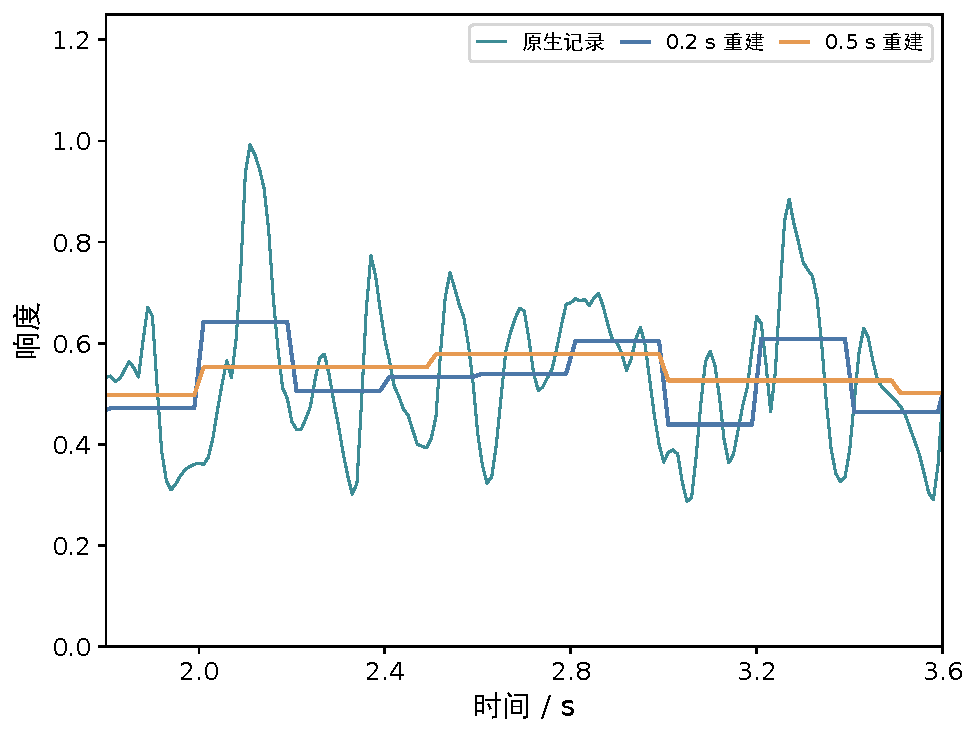
\includegraphics[width=\linewidth]{figures/fig_p1_window_reconstruction_single.pdf}
        \caption{响度的固定窗口聚合与重建}
        \label{fig:p1_window_reconstruction}
    \end{minipage}\hfill
    \begin{minipage}[b]{.48\linewidth}
        \centering
        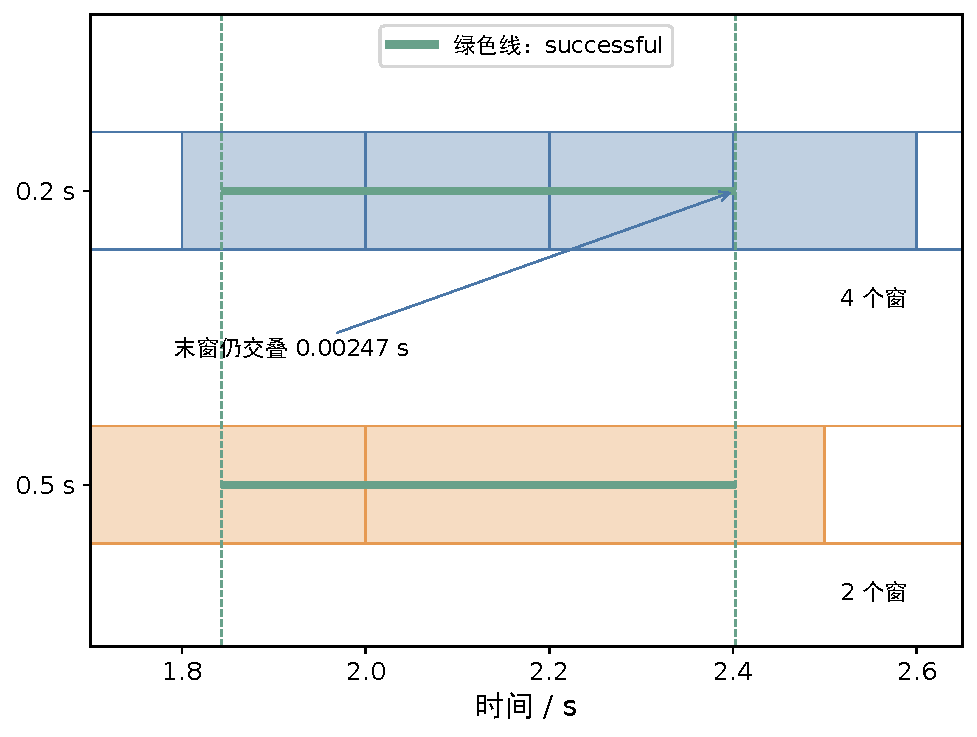
\includegraphics[width=\linewidth]{figures/fig_p1_word_window_overlap_single.pdf}
        \caption{候选词区间与固定窗口交叠}
        \label{fig:p1_word_window_overlap}
    \end{minipage}
\end{figure}

为判断上述现象是否仅出现在个别片段，本文对全量样本分别计算标准化重建均方误差与词跨界比例。重建误差将重建特征与原生特征之差按各维原生标准差归一化，再对有效记录和维度的平方误差取平均，数值越低表示越接近原生特征；仅纳入标准差大于$10^{-6}$的维度，有记录但全部维度恒定时记0，无有效记录时不计入模态均值。词跨界比例则在每条样本通过对齐筛选的词中，统计与至少两个窗口交叠的词所占比例，数值越高表示被切分的词越多。两类指标均先在样本内计算，再对相应有效样本等权平均，以区分特征变化的保留程度和词区间的完整性。

图~\ref{fig:p1_audio_window_error}至图~\ref{fig:p1_word_crossing_ratio}汇总全量对照。声学与视觉重建误差图中的短窗箱体整体低于长窗箱体，声学平均重建误差由0.7467降至0.5449，视觉由0.4373降至0.2357，相对降幅分别为27.02\%和46.10\%。图~\ref{fig:p1_word_crossing_ratio}则呈相反方向，平均词跨界比例由39.50\%升至71.33\%，增加31.83个百分点。三幅图分别基于100条声学样本、87条具有有效面部记录的样本和79条未触发整段复核的样本。图中菱形标出均值，箱内横线标出中位数，箱体覆盖第25至第75百分位数，须线延伸至1.5倍四分位距内的最远观测；箱外圆点仍参与统计。

\begin{figure}[H]
    \centering
    \begin{minipage}[b]{.32\linewidth}
        \centering
        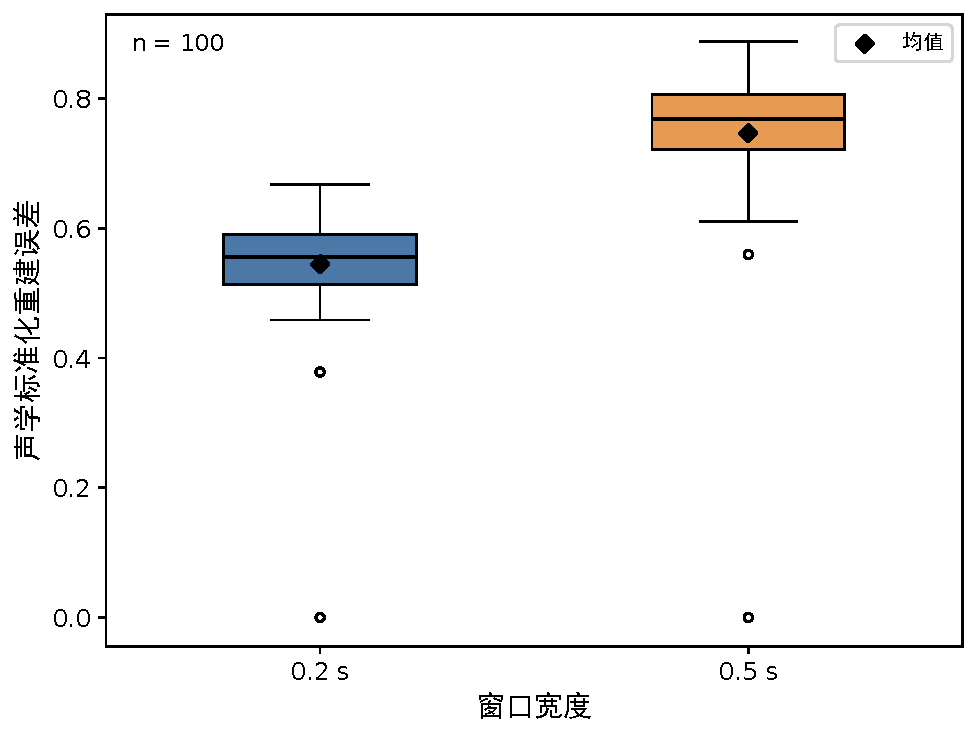
\includegraphics[width=\linewidth]{figures/fig_p1_audio_window_error_single.pdf}
        \caption{声学重建误差对照}
        \label{fig:p1_audio_window_error}
    \end{minipage}\hfill
    \begin{minipage}[b]{.32\linewidth}
        \centering
        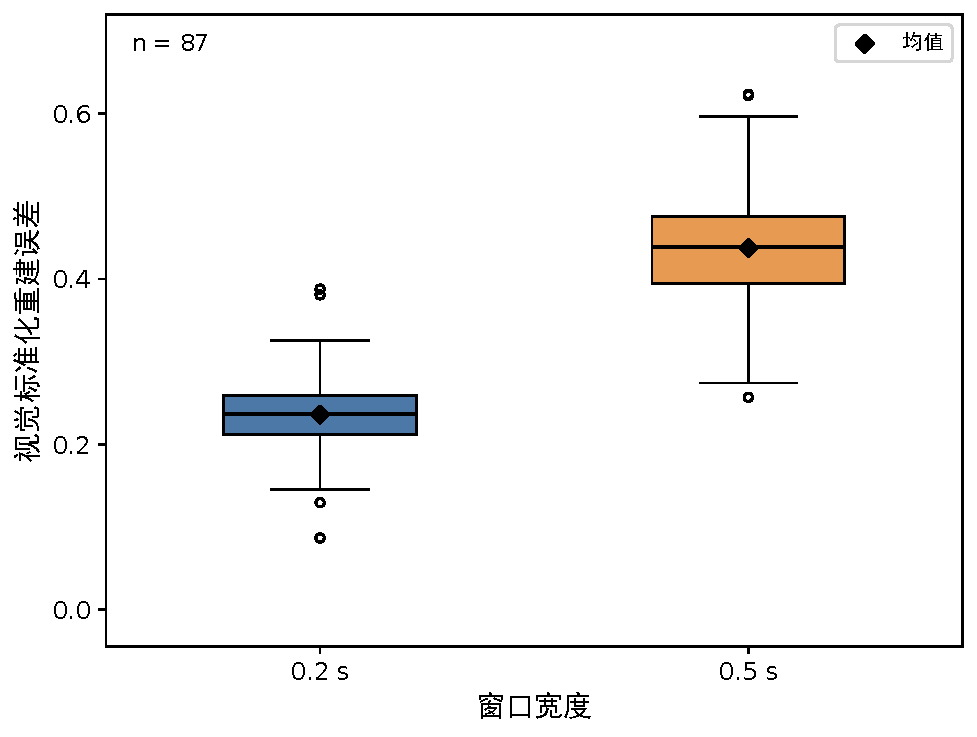
\includegraphics[width=\linewidth]{figures/fig_p1_vision_window_error_single.pdf}
        \caption{视觉重建误差对照}
        \label{fig:p1_vision_window_error}
    \end{minipage}\hfill
    \begin{minipage}[b]{.32\linewidth}
        \centering
        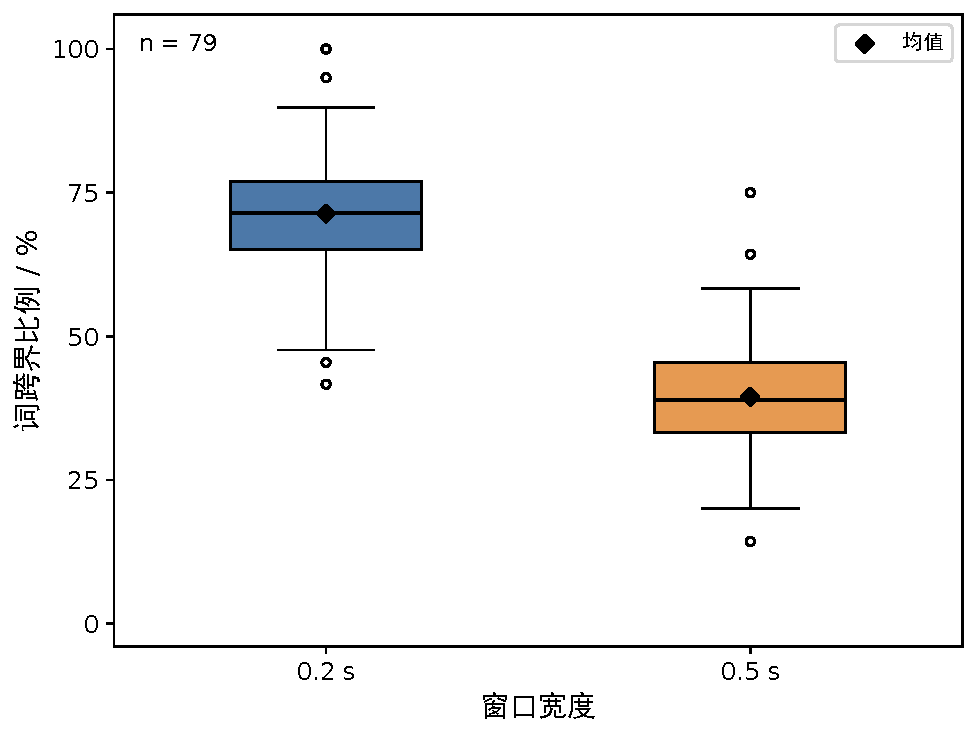
\includegraphics[width=\linewidth]{figures/fig_p1_word_crossing_ratio_single.pdf}
        \caption{词跨界比例对照}
        \label{fig:p1_word_crossing_ratio}
    \end{minipage}
\end{figure}

逐样本比较进一步表明，98条样本的短窗声学误差更低，另2条相同；87条样本的短窗视觉误差均更低；77条样本的短窗词跨界比例更高，另2条相同。两条声学误差相同的样本即前述全零音频样本，其特征不随时间变化，两种窗口的误差均按规则记0。将这两条样本单独列出后，其余98条样本的短窗、长窗平均声学误差分别为0.5560和0.7619，差异方向保持一致。

上述对照表明，在本次数据与窗口设置下，缩短窗口有利于保留原生特征的局部变化，却同时增加了词区间被固定边界切分的比例。因此，仅通过调整统一窗口宽度，仍需在这两个目标之间进行权衡。这一现象说明，以原文词为组织单位、再根据候选词区间聚合视听记录具有明确的任务动机：它使词级表示直接对应一个文本单元，并保留参与聚合的原生记录供回溯使用。不过，本实验未直接比较词级表示的重建误差，也未引入人工词界或情感预测任务，故不能据此断言词级表示在上述指标上优于固定窗口；其时间对应质量仍取决于候选词界及观测状态。

时间划分对照解释了聚合粒度的影响，而21条整段受限样本还涉及更基本的前提：给定英文转写是否具有相应的语音依据。若输入内容不对应，即使强制对齐能够生成完整路径，其候选词界也缺少真实发音支撑。为区分输入异常与一般的词界定位偏差，本文进一步对照实际音频和给定转写进行人工审核，按主要问题划分为表~\ref{tab:p1_manual_review}所列五类。各类互不重叠，共涉及317个原文词。

\begin{table}[H]
    \centering\small
    \caption{21条复核样本的人工审核结果}
    \label{tab:p1_manual_review}
    \setlength{\tabcolsep}{6pt}
    \renewcommand{\arraystretch}{1.12}
    \ifdefined\pOneCompactTableBox\else\newsavebox{\pOneCompactTableBox}\fi
    \begin{lrbox}{\pOneCompactTableBox}
    \begin{tabular}{lcc>{\raggedright\arraybackslash}p{18em}}
        \toprule
        审核发现 & 样本数 & 原文词数 & 主要表现\\
        \midrule
        音轨与文本不对应 & 11 & 120 & 实际语音内容与给定转写不对应\\
        无对应朗读 & 5 & 64 & 未听到对应朗读，其中1条为音乐\\
        非英语语音 & 3 & 93 & 实际语音并非英语\\
        分段内容不对应 & 1 & 18 & 前半段无朗读，后半段语音与转写不对应\\
        音频卡顿、局部对应 & 1 & 22 & 音频存在卡顿，部分词语与文本一致，但未形成完整对应\\
        \midrule
        合计 & 21 & 317 & \\
        \bottomrule
    \end{tabular}
    \end{lrbox}
    \usebox{\pOneCompactTableBox}
\end{table}

审核发现，音轨与文本不对应、缺少对应朗读等情况使给定转写缺少相应的语音依据；非英语语音则与所用英语声学模型及英文对齐目标不匹配。其中，3条非英语样本均来自视频\nolinkurl{-yRb-Jum7EQ}，两条全零音频样本归入“无对应朗读”。这些异常具有不同来源，不能统一解释为词界定位偏差。

样本\nolinkurl{-HwX2H8Z4hY$_$9}还说明了片段级检查的必要性。其平均词置信度为0.7238，仅9.09\%的词低于0.1，但诊断WER达到0.8636。人工审核发现音频存在卡顿，部分词语与转写一致，却没有形成完整逐词对应，说明局部得分较高不足以确认整段对应关系。

依据审核结果，本文维持这21条样本整体词级对应受限的标记，同时保留其原文、标签、原生特征与候选时间记录。该处理遵循题目关于保留原始样本并说明异常处理规则的要求，使内容对应异常能够被追溯，而不会通过修改转写或删除样本被隐去。由于本次审核未重建人工词界，不恢复局部词的对齐标记，前述筛选数量保持不变。审核范围仅为自动筛出的21条样本，不能据此认定其余79条均无异常，也不能计算全量词界准确率。

\subsubsection{典型样本的跨模态时序对齐验证}
\label{sec:p1_verification_examples}

全量统计明确了输出的使用范围，典型样本则进一步检验具体记录能否回溯到原始素材。本文继续采用样本\nolinkurl{-egA8-b7-3M$_$1}，展示文本片段、语音时段、视频帧及三类特征之间的对应。该样本给定转写包含“I started a successful Legal Nurse Consulting Business in 1989.”，图~\ref{fig:p1_multimodal_result}选取其中1.80--3.60~s的局部时段，自上而下排列实际画面、候选词区间、响度及面部系数。通过共同时间轴，可以从一个原文词定位其对应的声学记录与视频帧；其中浅绿底突出\texttt{successful}的候选区间，其内约2.11~s处出现响度峰值。图片按标注时刻定位，图片宽度不代表持续时间，面部曲线连线仅辅助观察。

\begin{figure}[H]
    \centering
    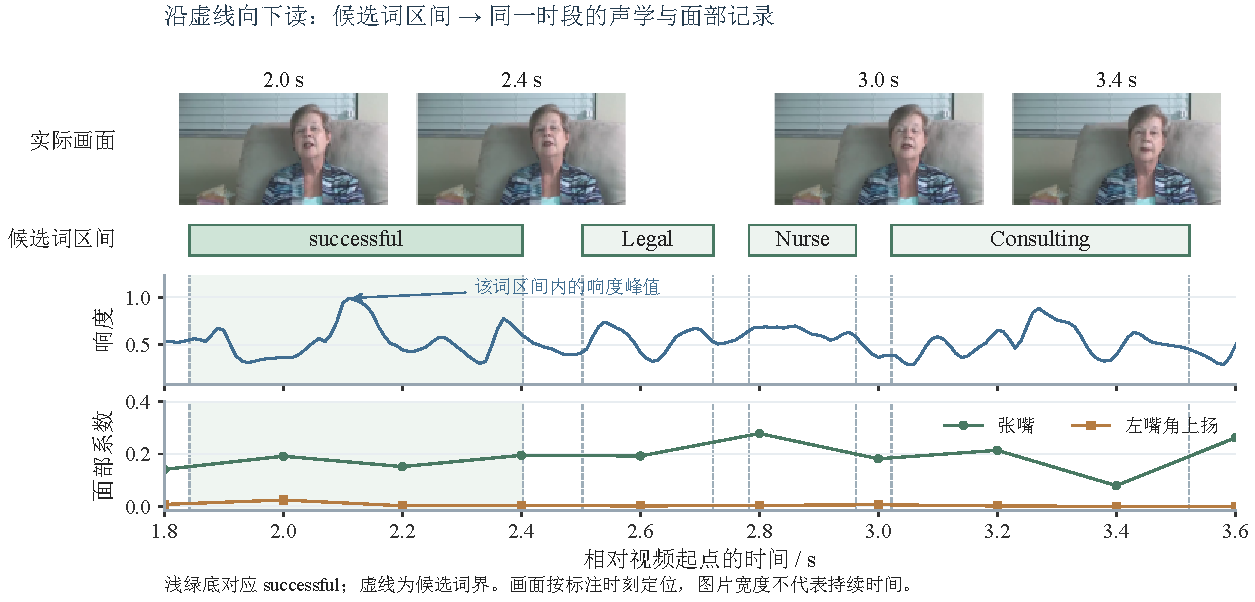
\includegraphics[width=\linewidth]{figures/fig_p1_multimodal_readable.pdf}
    \caption{词级映射的回溯示例：从候选词区间定位同一时段的声音与画面}
    \label{fig:p1_multimodal_result}
\end{figure}

表~\ref{tab:p1_mapping_records}列出部分映射记录。词\textit{successful}的候选区间为$[1.8425,2.4025]\,\mathrm{s}$，文本表示由子词索引3对应的隐藏向量获得，声学表示由183--240号共58条原生记录聚合，视觉表示由1.8、2.0、2.2、2.4~s四帧聚合。由此，该词的768维文本、25维声学与52维视觉向量均可回溯到各自来源。索引从0开始；声学索引指特征记录而非波形采样点，视觉帧依据时间支持区间参与聚合，因此帧中心可以位于词区间之外，边界帧的权重由实际交叠时长决定。

\begin{table}[H]
    \centering\small
    \caption{典型样本的部分词级映射记录}
    \label{tab:p1_mapping_records}
    \setlength{\tabcolsep}{6pt}
    \renewcommand{\arraystretch}{1.12}
    \ifdefined\pOneCompactTableBox\else\newsavebox{\pOneCompactTableBox}\fi
    \begin{lrbox}{\pOneCompactTableBox}
    \begin{tabular}{lcccc}
        \toprule
        原文词 & 子词索引 & 候选区间/s & 声学记录索引 & 视觉帧时刻/s\\
        \midrule
        started & 1 & $[1.2825,1.6425]$ & 127--164 & 1.2, 1.4, 1.6\\
        successful & 3 & $[1.8425,2.4025]$ & 183--240 & 1.8, 2.0, 2.2, 2.4\\
        Consulting & 6 & $[3.0225,3.5225]$ & 301--352 & 3.0, 3.2, 3.4, 3.6\\
        \bottomrule
    \end{tabular}
    \end{lrbox}
    \usebox{\pOneCompactTableBox}
\par\smallskip
\parbox{\wd\pOneCompactTableBox}{\footnotesize 注：索引从0开始；声学索引指具有正聚合权重的原生特征记录，不是波形采样点。视觉帧按其时间支持区间与候选词区间的交叠关系参与聚合，帧中心不必位于词区间内部。}
\end{table}

典型样本图与映射表共同展示了从原文词到模型子词、声学记录和视频帧的可追溯链条，使前文的聚合规则能够在具体输出上核验。进一步对全部100条样本独立复算交叠权重、视听聚合值和CTC置信度，重新计算诊断WER，并解码音视频核对时间记录与低能量标记，结果均在既定数值容差内与保存记录一致。这一检查验证了实现与既定计算规则的一致性；真实词界精度仍需人工时间标注评价。典型样本中的\texttt{in}和\texttt{1989}也继续保留置信度不足的标记，说明实例展示与质量筛选采用相同标准，没有因为选作典型样本而放宽使用条件。

\subsubsection{三模态特征文件说明与100条样本结果汇总}
\label{sec:p1_delivery}

以上统计与典型样本展示说明了输出的覆盖范围、质量状态和回溯方式。为进一步满足题目对自生成特征文件规范及全部100条样本结果汇总的要求，本文采用“统一模态规格＋逐样本明细”的组织方式：表~\ref{tab:p1_feature_specification}列出每条样本共有的模态类型、特征维数、矩阵形状与对齐粒度，表~\ref{tab:p1_all_samples}列出全部样本的编号、原始媒体时长及有效位置统计。两表结合，可确定任一样本三种模态的输出规格及使用范围；具体高维数值由相应样本目录中的特征文件提供。

\begin{table}[H]
    \centering\small
    \caption{三种模态的词级特征规格}
    \label{tab:p1_feature_specification}
    \setlength{\tabcolsep}{6pt}
    \renewcommand{\arraystretch}{1.12}
    \ifdefined\pOneCompactTableBox\else\newsavebox{\pOneCompactTableBox}\fi
    \begin{lrbox}{\pOneCompactTableBox}
    \begin{tabular}{lccc}
        \toprule
        模态 & 特征维数 & 样本矩阵形状 & 对齐粒度\\
        \midrule
        文本 & 768 & $L\times768$ & 原文词\\
        声学 & 25 & $L\times25$ & 原文词\\
        视觉（面部） & 52 & $L\times52$ & 原文词\\
        \bottomrule
    \end{tabular}
    \end{lrbox}
    \usebox{\pOneCompactTableBox}
\par\smallskip
\parbox{\wd\pOneCompactTableBox}{\footnotesize 注：$L$为对应样本的原文词数。各样本按实际词数存储，填充数与截断词数均为0；视觉模态不可观测的词位置采用零向量占位，并附无效标记。}
\end{table}

在时序组织上，每条样本按实际原文词数$L$保存变长序列，不进行统一长度填充或截断。$L$表示保留的词位置总数，模态观测有效位置数与通过对齐筛选的位置数另由掩码统计；这些位置不必连续，因此不能仅保存一个长度数值而省略逐位置标记。视觉无效位置的零向量用于在原词位置上占位，含义不同于在序列末尾追加的长度填充。

全量表中，“原文词数”对应三个矩阵的行数，“视觉可观测词数”统计能聚合有效面部记录的位置，“通过对齐筛选词数”依据前述两层筛选条件，最后一列为通过筛选且三种模态均可观测的词数。由于文本与声学在全部词位置均有可计算记录，最后一列等于对齐筛选与视觉可观测两个条件的交集。片段时长与音频时长均按前文的实际解码口径记录，用于定位原始媒体的时间范围，不将其解释为有效发声或面部可观测的累计时长。

例如，样本-s9qJ7ATP7w\$\_\$7共有28个词，其中14个视觉可观测，24个通过对齐筛选，同时满足两项条件的有12个。交集数量不能取前两项数量的较小值代替。

按上述口径，32条样本的全部词通过筛选且三种模态均可观测，46条样本仅部分词满足两项条件，1条样本的全部词通过对齐筛选但视觉模态不可观测，另21条样本经人工审核后整体词级对应仍受限。全量表按这四类依次排列，已审核的21条样本统一归入最后一类，各组互不重叠。

\begingroup
\small
\setlength{\tabcolsep}{6pt}
\renewcommand{\arraystretch}{1.12}
\setlength{\LTleft}{\fill}
\setlength{\LTright}{\fill}
\begin{longtable}{lrrrrrr}
\caption{附件1全部样本的特征输出与有效位置统计}\label{tab:p1_all_samples}\\
\toprule
样本编号 & \shortstack{片段\\时长/s} & \shortstack{音频\\时长/s} & \shortstack{原文\\词数} & \shortstack{视觉可观测\\词数} & \shortstack{通过对齐\\筛选词数} & \shortstack{其中三种模态\\都可观测\\词数}\\
\midrule
\endfirsthead
\multicolumn{7}{c}{表~\thetable\quad 特征输出与有效位置统计（续）}\\
\toprule
样本编号 & \shortstack{片段\\时长/s} & \shortstack{音频\\时长/s} & \shortstack{原文\\词数} & \shortstack{视觉可观测\\词数} & \shortstack{通过对齐\\筛选词数} & \shortstack{其中三种模态\\都可观测\\词数}\\
\midrule
\endhead
\midrule
\multicolumn{7}{r}{续下页}\\
\endfoot
\bottomrule
\endlastfoot
\multicolumn{7}{l}{\textbf{1. 全部词通过筛选且三种模态都可观测（32条）}}\\*
\nolinkurl{-3g5yACwYnA$_$3} & 14.389 & 14.328 & 29 & 29 & 29 & 29\\
\nolinkurl{-3nNcZdcdvU$_$5} & 7.868 & 7.789 & 18 & 18 & 18 & 18\\
\nolinkurl{-6rXp3zJ3kc$_$8} & 12.805 & 12.738 & 34 & 34 & 34 & 34\\
\nolinkurl{-I_e4mIh0yE$_$1} & 7.622 & 7.444 & 18 & 18 & 18 & 18\\
\nolinkurl{-I_e4mIh0yE$_$3} & 9.163 & 8.994 & 22 & 22 & 22 & 22\\
\nolinkurl{-MeTTeMJBNc$_$0} & 9.333 & 9.218 & 21 & 21 & 21 & 21\\
\nolinkurl{-MeTTeMJBNc$_$13} & 5.430 & 5.255 & 14 & 14 & 14 & 14\\
\nolinkurl{-RfYyzHpjk4$_$11} & 5.239 & 5.075 & 17 & 17 & 17 & 17\\
\nolinkurl{-RfYyzHpjk4$_$8} & 4.589 & 4.532 & 17 & 17 & 17 & 17\\
\nolinkurl{-UUCSKoHeMA$_$0} & 7.867 & 7.732 & 18 & 18 & 18 & 18\\
\nolinkurl{-UacrmKiTn4$_$10} & 7.362 & 7.242 & 18 & 18 & 18 & 18\\
\nolinkurl{-UacrmKiTn4$_$4} & 4.741 & 4.682 & 14 & 14 & 14 & 14\\
\nolinkurl{-aNfi7CP8vM$_$7} & 8.695 & 8.538 & 18 & 18 & 18 & 18\\
\nolinkurl{-aqamKhZ1Ec$_$0} & 11.000 & 10.890 & 14 & 14 & 14 & 14\\
\nolinkurl{-dxfTGcXJoc$_$1} & 16.161 & 16.018 & 37 & 37 & 37 & 37\\
\nolinkurl{-egA8-b7-3M$_$16} & 5.538 & 5.483 & 11 & 11 & 11 & 11\\
\nolinkurl{-egA8-b7-3M$_$17} & 7.271 & 7.095 & 16 & 16 & 16 & 16\\
\nolinkurl{-egA8-b7-3M$_$18} & 8.386 & 8.266 & 22 & 22 & 22 & 22\\
\nolinkurl{-egA8-b7-3M$_$20} & 6.645 & 6.474 & 20 & 20 & 20 & 20\\
\nolinkurl{-egA8-b7-3M$_$26} & 6.031 & 5.921 & 15 & 15 & 15 & 15\\
\nolinkurl{-egA8-b7-3M$_$6} & 6.265 & 6.183 & 12 & 12 & 12 & 12\\
\nolinkurl{-egA8-b7-3M$_$9} & 5.090 & 4.936 & 10 & 10 & 10 & 10\\
\nolinkurl{-mqbVkbCndg$_$0} & 6.500 & 6.386 & 14 & 14 & 14 & 14\\
\nolinkurl{-s9qJ7ATP7w$_$6} & 2.475 & 2.315 & 5 & 5 & 5 & 5\\
\nolinkurl{-s9qJ7ATP7w$_$8} & 3.295 & 3.184 & 12 & 12 & 12 & 12\\
\nolinkurl{-t217m2on-s$_$7} & 17.183 & 17.026 & 45 & 45 & 45 & 45\\
\nolinkurl{-tPCytz4rww$_$10} & 4.789 & 4.679 & 12 & 12 & 12 & 12\\
\nolinkurl{-tPCytz4rww$_$11} & 5.467 & 5.379 & 17 & 17 & 17 & 17\\
\nolinkurl{-tPCytz4rww$_$18} & 6.645 & 6.569 & 16 & 16 & 16 & 16\\
\nolinkurl{-uywlfIYOS8$_$4} & 6.045 & 5.881 & 18 & 18 & 18 & 18\\
\nolinkurl{-wny0OAz3g8$_$0} & 3.333 & 3.274 & 9 & 9 & 9 & 9\\
\nolinkurl{-wny0OAz3g8$_$2} & 6.687 & 6.523 & 23 & 23 & 23 & 23\\
\addlinespace[0.5em]
\multicolumn{7}{l}{\textbf{2. 部分词通过筛选且三种模态都可观测（46条）}}\\*
\nolinkurl{-3g5yACwYnA$_$13} & 5.514 & 5.399 & 15 & 15 & 14 & 14\\
\nolinkurl{-3g5yACwYnA$_$2} & 9.394 & 9.231 & 14 & 14 & 13 & 13\\
\nolinkurl{-3g5yACwYnA$_$9} & 8.817 & 8.696 & 23 & 23 & 21 & 21\\
\nolinkurl{-571d8cVauQ$_$0} & 5.167 & 4.992 & 12 & 12 & 10 & 10\\
\nolinkurl{-571d8cVauQ$_$5} & 15.273 & 15.115 & 43 & 43 & 42 & 42\\
\nolinkurl{-9y-fZ3swSY$_$0} & 6.900 & 6.757 & 22 & 22 & 19 & 19\\
\nolinkurl{-9y-fZ3swSY$_$4} & 2.821 & 2.665 & 9 & 9 & 6 & 6\\
\nolinkurl{-9y-fZ3swSY$_$8} & 4.989 & 4.917 & 12 & 3 & 11 & 2\\
\nolinkurl{-AUZQgSxyPQ$_$2} & 22.511 & 22.405 & 41 & 41 & 39 & 39\\
\nolinkurl{-HeZS2-Prhc$_$2} & 8.262 & 8.151 & 16 & 16 & 15 & 15\\
\nolinkurl{-HwX2H8Z4hY$_$2} & 3.982 & 3.916 & 7 & 1 & 4 & 1\\
\nolinkurl{-HwX2H8Z4hY$_$5} & 5.653 & 5.544 & 9 & 2 & 8 & 2\\
\nolinkurl{-HwX2H8Z4hY$_$6} & 3.358 & 3.256 & 7 & 5 & 6 & 5\\
\nolinkurl{-MeTTeMJBNc$_$7} & 10.517 & 10.411 & 31 & 31 & 29 & 29\\
\nolinkurl{-RfYyzHpjk4$_$2} & 5.516 & 5.392 & 25 & 24 & 21 & 21\\
\nolinkurl{-THoVjtIkeU$_$12} & 14.896 & 14.806 & 39 & 39 & 38 & 38\\
\nolinkurl{-THoVjtIkeU$_$2} & 4.292 & 4.231 & 10 & 10 & 9 & 9\\
\nolinkurl{-THoVjtIkeU$_$6} & 8.097 & 7.983 & 30 & 30 & 27 & 27\\
\nolinkurl{-UuX1xuaiiE$_$0} & 3.700 & 3.576 & 9 & 6 & 8 & 5\\
\nolinkurl{-UuX1xuaiiE$_$1} & 10.350 & 10.268 & 27 & 1 & 27 & 1\\
\nolinkurl{-UuX1xuaiiE$_$3} & 4.130 & 4.038 & 9 & 9 & 8 & 8\\
\nolinkurl{-UuX1xuaiiE$_$6} & 8.114 & 7.944 & 22 & 22 & 20 & 20\\
\nolinkurl{-a55Q6RWvTA$_$3} & 22.154 & 22.083 & 65 & 60 & 63 & 58\\
\nolinkurl{-dxfTGcXJoc$_$0} & 20.533 & 20.410 & 40 & 33 & 39 & 32\\
\nolinkurl{-dxfTGcXJoc$_$2} & 16.698 & 16.633 & 34 & 34 & 33 & 33\\
\nolinkurl{-dxfTGcXJoc$_$6} & 12.735 & 12.628 & 28 & 28 & 27 & 27\\
\nolinkurl{-egA8-b7-3M$_$1} & 10.266 & 10.156 & 20 & 20 & 18 & 18\\
\nolinkurl{-egA8-b7-3M$_$13} & 4.184 & 4.024 & 11 & 11 & 10 & 10\\
\nolinkurl{-lzEya4AM_4$_$5} & 7.675 & 7.570 & 19 & 19 & 18 & 18\\
\nolinkurl{-lzEya4AM_4$_$6} & 14.792 & 14.740 & 43 & 43 & 42 & 42\\
\nolinkurl{-qDkUB0GgYY$_$6} & 4.678 & 4.615 & 16 & 16 & 12 & 12\\
\nolinkurl{-s9qJ7ATP7w$_$0} & 6.867 & 6.711 & 24 & 24 & 23 & 23\\
\nolinkurl{-s9qJ7ATP7w$_$1} & 4.792 & 4.644 & 11 & 11 & 10 & 10\\
\nolinkurl{-s9qJ7ATP7w$_$4} & 4.427 & 4.247 & 9 & 6 & 8 & 5\\
\nolinkurl{-s9qJ7ATP7w$_$5} & 8.561 & 8.398 & 19 & 19 & 18 & 18\\
\nolinkurl{-s9qJ7ATP7w$_$7} & 6.966 & 6.839 & 28 & 14 & 24 & 12\\
\nolinkurl{-t217m2on-s$_$2} & 5.686 & 5.630 & 12 & 12 & 11 & 11\\
\nolinkurl{-tANM6ETl_M$_$3} & 6.758 & 6.604 & 22 & 22 & 21 & 21\\
\nolinkurl{-tPCytz4rww$_$12} & 11.864 & 11.736 & 26 & 26 & 24 & 24\\
\nolinkurl{-tPCytz4rww$_$16} & 7.206 & 7.139 & 16 & 16 & 14 & 14\\
\nolinkurl{-vxjVxOeScU$_$4} & 9.127 & 9.037 & 21 & 21 & 18 & 18\\
\nolinkurl{-wMB_hJL-3o$_$7} & 6.044 & 5.976 & 22 & 22 & 21 & 21\\
\nolinkurl{-wny0OAz3g8$_$3} & 6.146 & 6.100 & 20 & 1 & 20 & 1\\
\nolinkurl{-wny0OAz3g8$_$5} & 6.912 & 6.741 & 20 & 1 & 20 & 1\\
\nolinkurl{-wny0OAz3g8$_$7} & 8.068 & 7.910 & 29 & 6 & 29 & 6\\
\nolinkurl{-wny0OAz3g8$_$9} & 6.213 & 6.043 & 20 & 20 & 19 & 19\\
\addlinespace[0.5em]
\multicolumn{7}{l}{\textbf{3. 全部词通过对齐筛选，但视觉模态不可观测（1条）}}\\*
\nolinkurl{-wny0OAz3g8$_$1} & 6.844 & 6.777 & 22 & 0 & 22 & 0\\
\addlinespace[0.5em]
\multicolumn{7}{l}{\textbf{4. 整段对齐受限（已完成人工审核）（21条）}}\\*
\nolinkurl{-HwX2H8Z4hY$_$9} & 7.734 & 7.636 & 22 & 0 & 0 & 0\\
\nolinkurl{-NFrJFQijFE$_$1} & 5.746 & 5.659 & 16 & 0 & 0 & 0\\
\nolinkurl{-NFrJFQijFE$_$2} & 6.856 & 6.698 & 18 & 0 & 0 & 0\\
\nolinkurl{-hnBHBN8p5A$_$6} & 6.401 & 6.333 & 13 & 0 & 0 & 0\\
\nolinkurl{-hnBHBN8p5A$_$7} & 7.372 & 7.309 & 13 & 0 & 0 & 0\\
\nolinkurl{-iRBcNs9oI8$_$3} & 5.621 & 5.538 & 8 & 0 & 0 & 0\\
\nolinkurl{-iRBcNs9oI8$_$6} & 2.903 & 2.820 & 5 & 0 & 0 & 0\\
\nolinkurl{-iRBcNs9oI8$_$7} & 4.104 & 4.006 & 9 & 0 & 0 & 0\\
\nolinkurl{-iRBcNs9oI8$_$8} & 8.093 & 8.026 & 21 & 0 & 0 & 0\\
\nolinkurl{-iRBcNs9oI8$_$9} & 3.416 & 3.374 & 5 & 0 & 0 & 0\\
\nolinkurl{-mJ2ud6oKI8$_$1} & 6.103 & 6.054 & 13 & 0 & 0 & 0\\
\nolinkurl{-mJ2ud6oKI8$_$2} & 5.731 & 5.702 & 11 & 0 & 0 & 0\\
\nolinkurl{-mJ2ud6oKI8$_$6} & 2.257 & 2.228 & 5 & 5 & 0 & 0\\
\nolinkurl{-mJ2ud6oKI8$_$8} & 4.192 & 4.171 & 11 & 11 & 0 & 0\\
\nolinkurl{-mJ2ud6oKI8$_$9} & 7.033 & 6.909 & 22 & 22 & 0 & 0\\
\nolinkurl{-ri04Z7vwnc$_$0} & 2.807 & 2.763 & 8 & 0 & 0 & 0\\
\nolinkurl{-ri04Z7vwnc$_$2} & 6.027 & 5.913 & 16 & 8 & 0 & 0\\
\nolinkurl{-ri04Z7vwnc$_$5} & 3.545 & 3.440 & 8 & 8 & 0 & 0\\
\nolinkurl{-yRb-Jum7EQ$_$1} & 29.288 & 29.110 & 49 & 48 & 0 & 0\\
\nolinkurl{-yRb-Jum7EQ$_$5} & 13.169 & 13.045 & 25 & 25 & 0 & 0\\
\nolinkurl{-yRb-Jum7EQ$_$6} & 11.243 & 11.243 & 19 & 19 & 0 & 0\\
\end{longtable}
\endgroup

为使全量汇总能够落实到具体文件，本文按样本编号建立目录，采用NPZ保存数值数组，采用JSON保存原文、标签、特征定义和处理信息，并以CSV分别汇总样本、模态及词级记录。各文件内容见表~\ref{tab:p1_files}。这种组织方式将高维特征与其解释信息共同保存，使查询某条样本时能够同时取得特征值、原始来源和质量状态，而不是仅得到脱离时间记录的向量。

\begin{table}[H]
    \centering\small
    \caption{特征结果文件及其内容}
    \label{tab:p1_files}
    \setlength{\tabcolsep}{6pt}
    \renewcommand{\arraystretch}{1.12}
    \ifdefined\pOneCompactTableBox\else\newsavebox{\pOneCompactTableBox}\fi
    \begin{lrbox}{\pOneCompactTableBox}
    \begin{tabular}{l>{\raggedright\arraybackslash}p{24em}}
        \toprule
        文件 & 内容\\
        \midrule
        features.npz & 词级三模态矩阵、候选词区间、观测标记，以及原生视听特征和聚合权重。\\
        metadata.json & 原文、标签、词与子词位置、各维特征名称及处理参数。\\
        \nolinkurl{quality_masks.npz}、\newline quality.json & 对齐质量筛选结果、结合观测状态的有效位置标记及自动筛选原因。\\
        \nolinkurl{windows_0.2s.npz}、\newline\nolinkurl{windows_0.5s.npz} & 固定窗口边界、视听特征及文本聚合权重。\\
        人工审核\_21条样本.csv & 21条样本的人工审核状态、问题分类与原始说明。\\
        三份CSV汇总表 & \nolinkurl{sample_summary.csv}、\nolinkurl{modality_summary.csv}和\nolinkurl{word_alignment.csv}分别对应100条样本、300条样本--模态记录及1932个词的明细。\\
        \bottomrule
    \end{tabular}
    \end{lrbox}
    \usebox{\pOneCompactTableBox}
\end{table}

读取时，先通过样本编号定位目录，从\nolinkurl{features.npz}载入\nolinkurl{text}、\nolinkurl{audio}和\nolinkurl{vision}数组，相同行均对应同一原文词；再读取\nolinkurl{word_bounds}中的候选起止时间，并结合\nolinkurl{metadata.json}中的原文、词与子词记录解释该位置。用于词级视听分析时，还需读取\nolinkurl{quality_masks.npz}中的模态有效位置标记，例如\nolinkurl{vision_aligned_usable}取1表示该词通过对齐筛选且视觉可观测。保存的原生记录索引和聚合权重可用于复算词级向量，固定窗口的文本表示则由词权重与词级文本矩阵相乘获得。由此，样本编号、特征行、候选时间和原始素材之间形成可逐级核验的对应关系。

\subsubsection{方案可复现性说明}
\label{sec:p1_reproducibility}

为使前述处理结果能够复现，本文同时记录工具与模型版本、关键参数、配置文件、模型文件哈希及处理日志。实验环境和主要参数见表~\ref{tab:p1_repro_settings}；词级与片段级质量筛选条件已在时序对齐评估中明确列出。预训练模型用于冻结特征提取及声学对齐，不使用本问情感标签训练或微调，从而使本问的复现对象集中于输入处理、特征生成、时间映射与质量标记。

\begin{table}[H]
    \centering\small
    \caption{实验环境与主要参数}
    \label{tab:p1_repro_settings}
    \setlength{\tabcolsep}{6pt}
    \renewcommand{\arraystretch}{1.12}
    \ifdefined\pOneCompactTableBox\else\newsavebox{\pOneCompactTableBox}\fi
    \begin{lrbox}{\pOneCompactTableBox}
    \begin{tabular}{l>{\raggedright\arraybackslash}p{27em}}
        \toprule
        项目 & 版本或参数\\
        \midrule
        运行环境 & Python 3.10.13；PyTorch 2.5.1；CUDA 12.1。\\
        音视频读取 & PyAV 17.0.1；音频16 kHz、单声道；视频目标抽样频率5 Hz。\\
        文本编码 & Transformers 4.48.3；\nolinkurl{distilbert/distilbert-base-uncased}；每块最多510个子词，另加首尾标记。\\
        声学对齐 & \nolinkurl{facebook/wav2vec2-base-960h}；CTC最大概率路径。\\
        声学特征 & openSMILE 2.6.0；eGeMAPSv02的25维低层描述量。\\
        面部特征 & MediaPipe 0.10.21；Face Landmarker float16版本1；52维表情系数；检测与存在阈值均为0.5，最多两张脸，选择面积最大者。\\
        数值计算 & NumPy 1.26.4；SciPy 1.15.3；特征采用32位浮点数；num2words 0.5.14；随机种子20260923。\\
        \bottomrule
    \end{tabular}
    \end{lrbox}
    \usebox{\pOneCompactTableBox}
\end{table}

完整运行流程如下：首先依据环境清单和模型哈希准备相同的工具与权重，核对视频、转写和标签的样本标识，并进行媒体解码检查；随后完成文本规范化、音频重采样和带实际时间戳的视频抽样，分别提取三模态特征，估计CTC候选词区间，并按时间交叠聚合视听记录；最后生成质量标记、固定窗口对照和全量汇总，再独立复算时间映射与聚合结果。实际执行顺序、命令及异常记录随代码说明和日志保存，21条样本的人工审核说明单独保留，以区分程序计算结果与人工内容核查。

复现检查分别覆盖输入与实现的一致性、计算结果的一致性和重复提取的一致性。已有全量核验确认100条样本的源视频、处理代码、配置及模型文件哈希一致，候选路径与聚合结果符合既定规则；此外，将两条独立试跑样本与正式提取结果逐字段比较，特征的最大绝对差为0。前者覆盖全部样本的结构和计算核验，后者验证两条样本在相同条件下的重复提取结果，不将其扩大解释为全量重复运行或跨环境完全一致。上述记录与特征文件共同构成可复核、可复现的交付材料。

\subsection{本问小结}

本问完成了附件1全部100条样本的文本、声学与视觉特征提取，以词为共同组织单位，分别构建768维、25维和52维的变长词级表示。通过CTC强制对齐估计候选词区间，结合实际时间戳与时间交叠权重聚合有效视听观测，建立词级特征与原文、音频记录及视频帧之间的可追溯映射。全部1932个原文词均予以保留，其中1545个通过对齐质量筛选，占79.97\%；1387个同时通过筛选且三种模态均可观测，占全部词的71.79\%。对21条整段复核样本的人工审核进一步识别了内容对应异常，并据此维持其词级对应的使用限制。固定窗口对照显示，相较于0.5~s窗口，0.2~s窗口的重建误差更低，但词区间被切分的比例更高，体现了局部特征变化保留与词区间完整性之间的权衡。

该方案在保留全部样本及原始词位置的同时，分别记录观测有效性与对齐质量，使模态缺失和时间对应异常能够被独立识别。当前尚缺少人工词界标注，筛选通过比例不能解释为对齐准确率；约5~Hz的视频抽样对快速面部变化的表征有限，所选人脸未验证为说话者，视觉特征也未覆盖场景与肢体信息。因此，使用输出时应结合质量标记，并限定对特征含义与时间对应的解释范围。此外，本问提取的特征与附件2提供的768、74和35维特征在定义及维度配置上不同，后续各问仍应采用题目规定的特征输入，不能直接混用或替换。
